\documentclass[11pt]{article}

% Packages
\usepackage[utf8]{inputenc}
\usepackage{amsmath, amssymb}
\usepackage{graphicx}
\usepackage{hyperref}
\usepackage{geometry}
\usepackage{authblk}
\usepackage{natbib}
\usepackage{setspace}
\usepackage{float}
\usepackage{booktabs}

% Page setup
\geometry{margin=1in}
\onehalfspacing

% Title and Author Info
\title{\textbf{Tipping the Climate Equilibrium: Tensor-Based Game Theory for Identifying Critical Coalitions in Climate Policy Negotiations}}

\date{}

\newcommand{\keywords}[1]{\par\noindent\textbf{Keywords:} #1}

\begin{document}

\maketitle

\begin{abstract}
We introduce a tensor-based extension of multiplayer game theory to model how small coalitions of relatively low-influence actors can tip the equilibrium in climate policy negotiations. Traditional game-theoretic approaches struggle to capture the high-dimensional, nonlinear, and asymmetric nature of international climate interactions. Our formulation represents strategic influence as a third-order tensor $\mathcal{T} \in \mathbb{R}^{N \times N \times N}$, where each entry quantifies the joint influence of two actors on a third, and defines a tipping score to identify coalitions capable of shifting systemic outcomes through coordinated cooperation.

We prove formally that for the real-data influence tensor the first-order Z-eigenvalue shift under coalition activation equals a weighted combination of internal co-ratification alignment and outward influence spread, providing an exact algebraic grounding for the tipping score metric. We validate the framework analytically on small synthetic systems, demonstrating eigenvalue-driven phase transitions when minor-player coalitions are activated, and computationally on a real-data pipeline covering 175 non-G20 nations across 263 multilateral environmental agreements (1950--2017). Vulnerability scores from the ND-GAIN Country Index and WRI Aqueduct 4.0 are integrated into the reward function, creating an incentive for including frontline-affected nations in optimal coalitions. A REINFORCE policy gradient agent using Gumbel top-$K$ sampling discovers coalitions that outperform exhaustive random search by 14.7\%, achieving a peak tipping score of 22,229 across 4,964 unique configurations. Keystone country analysis identifies Uruguay, Tunisia, Greece, and Algeria as consistently high-leverage coalition anchors. We find that cross-cluster geographic diversity spanning at least 6 of 8 treaty-participation clusters is a necessary condition for top-scoring coalitions, consistent with the theoretical expectation that high-leverage coalitions tend to span geographically and institutionally disparate treaty communities.
\end{abstract}

\keywords{tensor games; coalition formation; climate negotiations; reinforcement learning; Z-eigenvalue; tipping points}

\section{Introduction}
\label{sec:intro}

Climate change negotiations involve numerous heterogeneous actors --- from nation-states to regional coalitions and private sector alliances. Despite large-scale asymmetries in power and emissions, small coalitions have repeatedly shifted global momentum in ways that aggregate power metrics would not predict. The Alliance of Small Island States, representing under 1\% of global emissions, helped anchor the 1.5\textdegree C temperature goal in the Paris Agreement. The High Ambition Coalition catalysed ambitious transparency language across a far larger set of parties. Understanding \emph{which} small coalitions carry this kind of systemic leverage, and why, is a question that existing game-theoretic frameworks have not satisfactorily addressed.

Standard cooperative game theory identifies stable allocations and pivotal players, but is not designed to model dynamic influence propagation through a heterogeneous network. Non-cooperative Nash equilibrium models assume symmetric information and discrete action spaces ill-suited to the continuous, norm-driven adjustment of multilateral diplomacy. We propose that the interaction structure of climate negotiations is fundamentally triadic: each country's strategic update depends not on bilateral relationships alone, but on how \emph{pairs} of other actors jointly shape the normative environment. Third-order tensors are the natural representation for this structure.

This paper makes the following contributions:
\begin{enumerate}
    \item A formal tensor-based dynamical model of climate strategy interactions, with analytical conditions for coalition-induced tipping (Sections~\ref{sec:math}--\ref{sec:simulation}).
    \item A hierarchical clustering analysis of 175 non-G20 nations across 263 multilateral treaties, identifying eight treaty-participation communities and motivating cross-cluster coalition search (Section~\ref{sec:clustering}).
    \item A real-data pipeline integrating treaty participation, ND-GAIN vulnerability, and WRI Aqueduct water stress data for 175 non-G20 nations, with a corrected country-name resolver ensuring consistent joins across heterogeneous datasets (Section~\ref{sec:results_realdata}).
    \item A REINFORCE policy gradient agent using Gumbel top-$K$ sampling that scales coalition discovery to $N=175$ without the reward sparsity problems of Bernoulli-based approaches, achieving a 14.7\% improvement over random search (Section~\ref{sec:results_realdata}).
\end{enumerate}

The paper is organised as follows. Section~\ref{sec:background} provides empirical motivation. Section~\ref{sec:related} reviews related work. Section~\ref{sec:math} presents the mathematical framework, including the derivation of TippingScore as a tractable proxy for the Z-eigenvalue bifurcation criterion (Section~\ref{sec:tipping_score_proxy}). Sections~\ref{sec:simulation} and~\ref{sec:clustering} describe simulation experiments and clustering analysis respectively. Section~\ref{sec:results_realdata} presents real-data results. Section~\ref{sec:discussion} discusses implications and limitations, and Section~\ref{sec:conclusion} concludes.

\section{Background and Motivation}
\label{sec:background}

International climate negotiations operate across two distinct timescales. On the longer scale, formal agreements such as the Kyoto Protocol (1997) and the Paris Agreement (2015) establish binding or voluntary emissions commitments among all UNFCCC parties. On the shorter scale, specific negotiation rounds are shaped by informal diplomatic coalitions that advocate for particular positions, draft text, and build political momentum. The history of these negotiations reveals a recurring pattern: small, strategically assembled coalitions of relatively low-power nations have repeatedly outperformed their nominal influence, shifting outcomes in ways that larger blocs could not.

The Alliance of Small Island States (AOSIS) is perhaps the most cited example. Despite representing fewer than 1\% of global greenhouse gas emissions, AOSIS was instrumental in establishing the 1.5\textdegree C aspirational target in the Paris Agreement, a position far from settled at the outset of COP21~\cite{aosis2023}. Similarly, the High Ambition Coalition, a cross-regional grouping of approximately 100 parties, emerged during COP21 to push for ambitious language on long-term temperature goals and transparency mechanisms. These cases illustrate that coalition effectiveness depends not on aggregate emissions or economic power, but on alignment, geographic diversity, and strategic timing.

This observation raises a formal question: given the multi-dimensional strategic landscape of climate negotiations, which properties characterise small coalitions with disproportionate influence? Standard approaches from cooperative game theory, such as Shapley values and core analysis, address payoff allocation but are not designed to model the dynamic propagation of influence through a heterogeneous network of actors. Non-cooperative approaches based on Nash equilibrium assume symmetric information and well-defined action spaces that do not naturally accommodate the continuous, norm-driven adjustment observed in multilateral diplomacy~\cite{barrett1994self, nordhaus2015climate}.

We argue that the interaction structure in climate negotiations is fundamentally triadic: a country's strategic update depends not only on bilateral relationships but on how \emph{pairs} of other actors jointly influence the normative landscape. This is the structure captured by third-order tensors. By representing influence as a tensor $\mathcal{T} \in \mathbb{R}^{N \times N \times N}$, we can model nonlinear coalition dynamics that bilateral frameworks miss. Combined with a reinforcement learning policy gradient optimiser trained on real treaty participation data, this approach provides a computationally tractable method for identifying candidate tipping coalitions from the full space of non-G20 nations.

\section{Related Work}
\label{sec:related}

Climate change negotiations have long been studied through the lens of game theory, particularly in the context of public goods and cooperative behaviour among sovereign actors. Early work in this field focused on repeated games and Nash equilibrium approaches, assuming rational actors with symmetric incentives \citep{barrett1994self, nordhaus2015climate}. However, these frameworks often fall short when modelling heterogeneous influence, asymmetric stakes, and dynamic tipping behaviours.

\citet{tavoni2009coalitions} introduced the idea of coalition formation games with spillover effects, where smaller groups of actors could lead in technology adoption and thereby reduce the costs of mitigation for non-participants. This resonates with real-world developments, such as the EU’s leadership in carbon pricing and the influence of subnational actors post-Kyoto.

Roemer’s \textit{Kantian equilibrium} framework \citep{roemer2010kantian} also shifts the focus from traditional utility-maximising behaviour to principled cooperative norms, offering a route to understand policy emergence when actors care about global outcomes. In a similar vein, \citet{young2015individual} and others have explored the role of social norms, tipping points, and behavioural diffusion in large-scale coordination problems.

On the computational side, tensor methods have seen increasing application in multi-agent systems and generalised games \citep{cheng2014tensor}, but have yet to be widely adopted in the domain of environmental policy modelling. Our work bridges this gap by combining high-dimensional tensor representations with coalition tipping logic, and applies this hybrid to the analysis of catalytic influence in climate negotiations.

\paragraph{Treaty regime formation and the decisional logic of membership.}
\citet{cope2025decisional} develops a formal model of treaty regime formation in which each state's membership decision depends on the bilateral marginal value $v_j$ contributed by every incumbent member, modulated by an externality parameter $e \in [0,1]$ that governs how much of the regime's benefits spill to non-members. This bilateral utility structure --- where $i$'s decision depends on pairwise relationships with each existing member $j$ --- is a special case of the triadic interaction structure formalised by our influence tensor. In Cope's framework the joint effect of two members $j$ and $k$ on $i$ factorises into independent bilateral terms; in the general formulation of Section~\ref{sec:math}, $\mathcal{T}_{ijk}$ can capture a genuinely triadic effect that need not factorise. The real-data proxy of Section~\ref{sec:tipping_score_proxy}, $\mathcal{T}_{ijk} = \mathbf{x}_j \cdot \mathbf{x}_k$, does not exploit this generality: that entry is independent of $i$, so the proxy is bilateral in the same sense as Cope's framework, applied uniformly across recipients. Its value lies in tractability and direct connection to treaty co-ratification data rather than in modelling recipient-specific triadic effects. Treaty co-ratification $M_{jk} = \mathbf{x}_j \cdot \mathbf{x}_k$ serves as a proxy for the joint normative engagement that members $j$ and $k$ contribute to the strategic environment, and $\mathrm{InfluenceSpread}(C) = \sum_{j \in C,\, k \notin C} M_{jk}$ provides a computational counterpart to Cope's externality: a coalition with high InfluenceSpread projects strong normative pressure on non-member states, precisely the mechanism Cope's high-$e$ regime triggers. The two frameworks address complementary questions --- Cope asks which coalitions form stably under rational membership incentives; we ask which coalitions, once formed, maximise systemic tipping potential. Future work could use Cope's stability conditions as a feasibility filter on our coalition search, retaining candidates that are both high-scoring and rationalisable under his membership utility.

The present paper adds a third-order tensor layer to this literature, formally connecting spectral bifurcation conditions to a tractable coalition scoring rule and testing it on real treaty participation data.


\section{Mathematical Framework}
\label{sec:math}

We present a tensor-based dynamical model to describe strategic interactions among heterogeneous players in climate policy negotiations. This framework incorporates both asymmetric influence and nonlinear coalition dynamics to identify policy tipping points.

\subsection{Players, Strategies, and Influence}

Let there be $N$ players (e.g., countries or blocs) indexed by $i = 1, \dots, N$. Each player chooses a strategy $s_i \in [0,1]$ representing its level of climate cooperation, such as its commitment to emission reduction. Players are divided into two classes:
\begin{itemize}
	\item \textbf{Major players}: High influence actors (e.g., G7, BRICS)
	\item \textbf{Minor players}: Lower influence actors (e.g., island nations, smaller economies)
\end{itemize}

We define a third-order influence tensor $\mathcal{T} \in \mathbb{R}^{N \times N \times N}$, where $\mathcal{T}_{ijk}$ quantifies the influence that the joint strategies of players $j$ and $k$ have on the strategic update of player $i$. Entries of $\mathcal{T}$ are designed such that:
\begin{itemize}
	\item $\mathcal{T}_{ijk}$ is larger when $j$ or $k$ is a major player.
	\item Diagonal and self-influence terms (e.g., $\mathcal{T}_{iii}$) represent internal feedback.
\end{itemize}

\subsection{Dynamical System and Strategy Evolution}

The strategy dynamics for player $i$ are governed by the equation:
\begin{equation}
	\frac{ds_i}{dt} = -s_i + \sigma\left( \sum_{j,k=1}^{N} \mathcal{T}_{ijk} s_j s_k + \theta_i \right),
	\label{eq:dynamics}
\end{equation}
where:
\begin{itemize}
	\item $\sigma(x) = \frac{1}{1 + e^{-x}}$ is a sigmoid activation function modelling bounded rationality.
	\item $\theta_i$ is the intrinsic bias of player $i$, capturing internal incentives, such as economic self-interest, cost of mitigation, or political resistance.
	\item The term $-s_i$ ensures decay to the neutral strategy in absence of positive influence.
\end{itemize}

\subsection{Equilibrium and Stability Analysis}

A steady state of the system satisfies:
\begin{equation}
	\frac{ds_i}{dt} = 0 \quad \forall i.
\end{equation}

To assess the stability of equilibria, we consider the spectral properties of the tensor $\mathcal{T}$. In particular, we analyse the dominant \textit{Z-eigenvalue} $\lambda_{\max}$ of $\mathcal{T}$:
\begin{equation}
	\mathcal{T} \cdot \vec{s}^2 = \lambda \vec{s},
\end{equation}
where the tensor-vector contraction is performed on the last two modes, and $\vec{s}^2$ denotes element-wise squaring.

A large $\lambda_{\max}$ indicates that small perturbations can lead to systemic shifts — a signature of susceptibility to tipping.

\subsection{Critical Coalitions and Tipping Points}

Let $C \subset \{i \mid i \text{ is a minor player} \}$ be a proposed coalition. We define a \textit{perturbed strategy profile} by setting $s_c = 1$ for all $c \in C$ (full cooperation), while others evolve dynamically.

We define a modified influence tensor $\mathcal{T}^{(C)}$, in which the terms involving members of $C$ are amplified to reflect their coordinated influence:
\[
\mathcal{T}^{(C)}_{ijk} = 
\begin{cases}
	\eta \cdot \mathcal{T}_{ijk}, & \text{if } j \in C \text{ or } k \in C, \\
	\mathcal{T}_{ijk}, & \text{otherwise},
\end{cases}
\]
where $\eta > 1$ is the amplification factor (e.g., from alignment, bloc voting, technology sharing).

We seek the smallest coalition $C$ such that the perturbed tensor $\mathcal{T}^{(C)}$ causes a bifurcation in the system, defined as a qualitative shift in the equilibrium state of $\vec{s}$.

\subsection{Bifurcation and Tipping Threshold}

Let $\lambda_{\max}^{(C)}$ be the dominant Z-eigenvalue of $\mathcal{T}^{(C)}$. We define a tipping point when:
\[
\lambda_{\max}^{(C)} > \lambda_c,
\]
where $\lambda_c$ is a critical threshold empirically or analytically determined (e.g., from a saddle-node bifurcation analysis). The minimal cardinality of $C$ such that this holds defines a \textbf{critical coalition}.

\subsection{Algorithm for Identifying Critical Coalitions}

We propose the following method:

\begin{enumerate}
	\item \textbf{Tensor Construction}: Construct $\mathcal{T}$ from influence scores, using empirical data or network centrality (e.g., PageRank, betweenness).
	\item \textbf{Coalition Search}: For candidate sets $C$, evaluate $\lambda_{\max}^{(C)}$ using tensor contraction and spectral analysis.
	\item \textbf{Optimisation}: Apply a greedy or metaheuristic algorithm (e.g., simulated annealing) to identify the minimal $C$ for which $\lambda_{\max}^{(C)} > \lambda_c$.
	\item \textbf{Simulation}: Use the dynamical system \eqref{eq:dynamics} to simulate the evolution of strategies under the influence of coalition $C$.
\end{enumerate}

These four steps are implemented for small systems in Section~\ref{sec:simulation} and scaled to $N=175$ via TippingScore in Sections~\ref{sec:minor_coalitions}--\ref{sec:results_realdata}.

\subsection{Real-Data Approximation: TippingScore as a Tractable Proxy}
\label{sec:tipping_score_proxy}

For empirical applications at scale ($N \gg 10$), exact Z-eigenvalue computation is computationally intractable: the problem is NP-hard for general tensors~\citep{hillar2013most}. We therefore define the real-data influence tensor explicitly and derive a tractable scoring function that preserves the structural motivation of the bifurcation criterion.

\paragraph{Real-data tensor construction.}
Let $\mathbf{x}_i \in \{0,1\}^T$ be the binary treaty ratification vector of country $i$ across $T$ agreements. We define:
\begin{equation}
    \mathcal{T}_{ijk} = \mathbf{x}_j \cdot \mathbf{x}_k,
    \label{eq:real_tensor}
\end{equation}
where $\mathbf{x}_j \cdot \mathbf{x}_k$ counts treaties jointly ratified by $j$ and $k$, interpreted as the bilateral co-engagement strength of the sending pair $(j,k)$. Crucially, this entry is \emph{independent of the recipient index $i$}: setting $M = XX^\top$ (with $X$ the $N \times T$ ratification matrix, rows $\mathbf{x}_i^\top$), the proxy satisfies $\mathcal{T}_{ijk} = M_{jk}$ for every $i$. The tensor is therefore rank-1 in its first mode --- a deliberate simplification that replaces the fully recipient-specific triadic tensor of Sections~\ref{sec:math}--\ref{sec:simulation} with a tractable bilateral co-ratification structure in which influence depends only on the engagement of the sending pair, not on the identity of the recipient. The tensor is symmetric in its last two indices ($\mathcal{T}_{ijk} = \mathcal{T}_{ikj}$) and is consistent with the general formulation in Equation~\eqref{eq:dynamics}. For a coalition $C$ with $s_j = 1$ for $j \in C$ and $s_j = 0$ otherwise, the aggregate influence received by any country $i$ is:
\begin{equation}
    \left(\mathcal{T} \cdot \mathbf{s}_C^2\right)_i = \sum_{j,k \in C} M_{jk} = \left\|\sum_{j \in C} \mathbf{x}_j\right\|^2,
\end{equation}
identical for all $i$ (inside and outside the coalition alike). A shift in $\lambda_{\max}^{(C)}$ sufficient to trigger the bifurcation condition therefore depends on: (i) the internal co-ratification coherence of the coalition's treaty vectors, (ii) the aggregate outward treaty overlap from coalition members to non-members, and (iii) the structural diversity of the coalition's influence channels across distinct treaty communities (a heuristic criterion, motivated below).

\paragraph{TippingScore definition.}
We operationalise these three properties as:
\begin{align}
    \text{Alignment}(C) &= \frac{1}{|C|(|C|-1)} \sum_{\substack{j,k \in C \\ j \neq k}} \frac{\mathbf{x}_j \cdot \mathbf{x}_k}{\|\mathbf{x}_j\|\,\|\mathbf{x}_k\|}, \label{eq:alignment} \\
    \text{InfluenceSpread}(C) &= \sum_{\substack{i \in C,\, j \notin C}} M_{ij}, \quad M = XX^\top, \label{eq:spread} \\
    \text{ClusterDiversity}(C) &= \bigl|\{c(i) : i \in C\}\bigr|, \label{eq:diversity}
\end{align}
where $M_{ij} = \mathbf{x}_i \cdot \mathbf{x}_j$ is the bilateral treaty co-ratification count and $c(i)$ is the cluster assignment of country $i$. The composite score is:
\begin{equation}
    \text{TippingScore}(C) = \text{Alignment}(C) \times \text{InfluenceSpread}(C) \times \text{ClusterDiversity}(C).
    \label{eq:tipping_score}
\end{equation}

\paragraph{Proposition 1 (Z-eigenvalue structure of the proxy tensor).}
Assume $X \neq 0$. For the proxy tensor $\mathcal{T}_{ijk} = M_{jk}$, the contraction
\[
(\mathcal{T} \cdot s^2)_i = \sum_{j,k} M_{jk}\,s_j s_k = s^\top M s \;\geq\; 0
\]
is constant in $i$ and non-negative for every $s$. Consequently:
\begin{enumerate}
\item The uniform vector $s^* = \mathbf{1}/\sqrt{N}$ is a Z-eigenvector with eigenvalue $\lambda_0 = N^{-1/2}\sum_{j,k}M_{jk} > 0$.
It is the unique positive-valued unit Z-eigenvector up to sign and is therefore the \textbf{dominant Z-eigenvector} of $\mathcal{T}$.
\item Any unit vector $v \in \ker(X^\top)$ satisfies $\mathcal{T}\cdot v^2 = 0 = 0\cdot v$ and is a Z-eigenvector with eigenvalue $0$.
Such vectors exist whenever $\mathrm{rank}(X) < N$; if $\mathrm{rank}(X) = N$, then $\pm s^*$ are the only Z-eigenvectors.
No Z-eigenvector with negative eigenvalue exists, since $s^\top M s \geq 0$ for all $s$.
\end{enumerate}
Under the coalition perturbation $\mathcal{T}^{(C)}(\eta) = \mathcal{T} + (\eta-1)\Delta\mathcal{T}^{(C)}$ of Section~\ref{sec:math}, the dominant Z-eigenvalue satisfies:
\begin{equation}
    \frac{d\lambda_{\max}^{(C)}}{d\eta}\bigg|_{\eta=1} = \frac{1}{\sqrt{N}}\bigl[\mathrm{InternalSpread}(C) + 2\,\mathrm{InfluenceSpread}(C)\bigr],
    \label{eq:eigenvalue_sensitivity}
\end{equation}
where $\mathrm{InternalSpread}(C) = \sum_{j,k \in C} M_{jk}$ and $\mathrm{InfluenceSpread}(C)$ is as in Equation~\eqref{eq:spread}. The derivation differentiates the eigenvalue equation at $\eta=1$, using the $i$-independence of $\mathcal{T}$ to show that the Jacobian of $s \mapsto \mathcal{T}\cdot s^2$ at $s^*$ maps $\mathbb{R}^N$ into $\mathrm{span}(\mathbf{1})$, forcing the first-order eigenfunction perturbation to vanish ($s' = 0$). The eigenvalue shift then reduces to $(s^*)^\top[\Delta\mathcal{T}^{(C)}\cdot(s^*)^2]$, evaluated by inclusion-exclusion on the support $\{(j,k) : j \in C \text{ or } k \in C\}$ of $\Delta\mathcal{T}^{(C)}$ and symmetry of $M$.

Proposition~1 establishes a formal link between TippingScore and the eigenvalue bifurcation criterion \emph{for the proxy tensor at the dominant equilibrium $s^*$}. $\mathrm{InfluenceSpread}(C)$ appears explicitly in Equation~\eqref{eq:eigenvalue_sensitivity}, and $\mathrm{InternalSpread}(C) = \sum_{j,k\in C}M_{jk}$ is monotonically increasing in $\mathrm{Alignment}(C)$ when coalition members have comparable treaty engagement (equal $\|\mathbf{x}_j\|$). The $\mathrm{ClusterDiversity}$ multiplier in Equation~\eqref{eq:tipping_score} does \emph{not} follow from Equation~\eqref{eq:eigenvalue_sensitivity}; it is a heuristic design criterion that penalises configurations concentrating all coalition members within a single treaty community. The motivation is that coalitions with near-orthogonal ratification profiles exert influence through statistically independent channels, contributing to eigenvalue perturbations beyond the uniform equilibrium $s^*$; including $\mathrm{ClusterDiversity}$ as a multiplicative factor operationalises this intuition without formal derivation from the eigenvalue analysis.

While TippingScore is therefore not equivalent to $\Delta\lambda_{\max}^{(C)}$ for an arbitrary equilibrium $s^*$, it encodes the same structural criteria as the formal result: high-scoring coalitions are precisely those whose activation would produce the largest, most coherent, and most channel-diverse perturbation to the proxy tensor dynamics. The toy-system eigenvalue experiments in Section~\ref{sec:simulation} demonstrate the direct connection in the tractable ($N \leq 10$) regime; Sections~\ref{sec:minor_coalitions}--\ref{sec:results_realdata} apply TippingScore as the operational criterion at $N = 175$.


\section{Simulation and Interpretation}
\label{sec:simulation}

To demonstrate the behaviour of the proposed tensor-based climate strategy model, we simulate two scenarios of increasing complexity: a small illustrative system and a scalable extended setup that allows us to test tipping and learning hypotheses.

\subsection{Critical Coalition Tipping in a Small System}

We begin with a five-player system ($N=5$), where players 0 and 1 are designated as major actors with disproportionately large influence values in the tensor $\mathcal{T}$, while players 2--4 are minor actors with lower impact.

Two scenarios are simulated:
\begin{enumerate}
	\item \textbf{Baseline:} All players start with low cooperation, and no coordinated action occurs.
	\item \textbf{Minor Coalition Activated:} Players 3 and 4 are forced into full cooperation ($s_3 = s_4 = 1$), and their influence terms in the tensor are amplified by a factor $\eta = 2.5$.
\end{enumerate}

\begin{figure}[htbp]
	\centering
	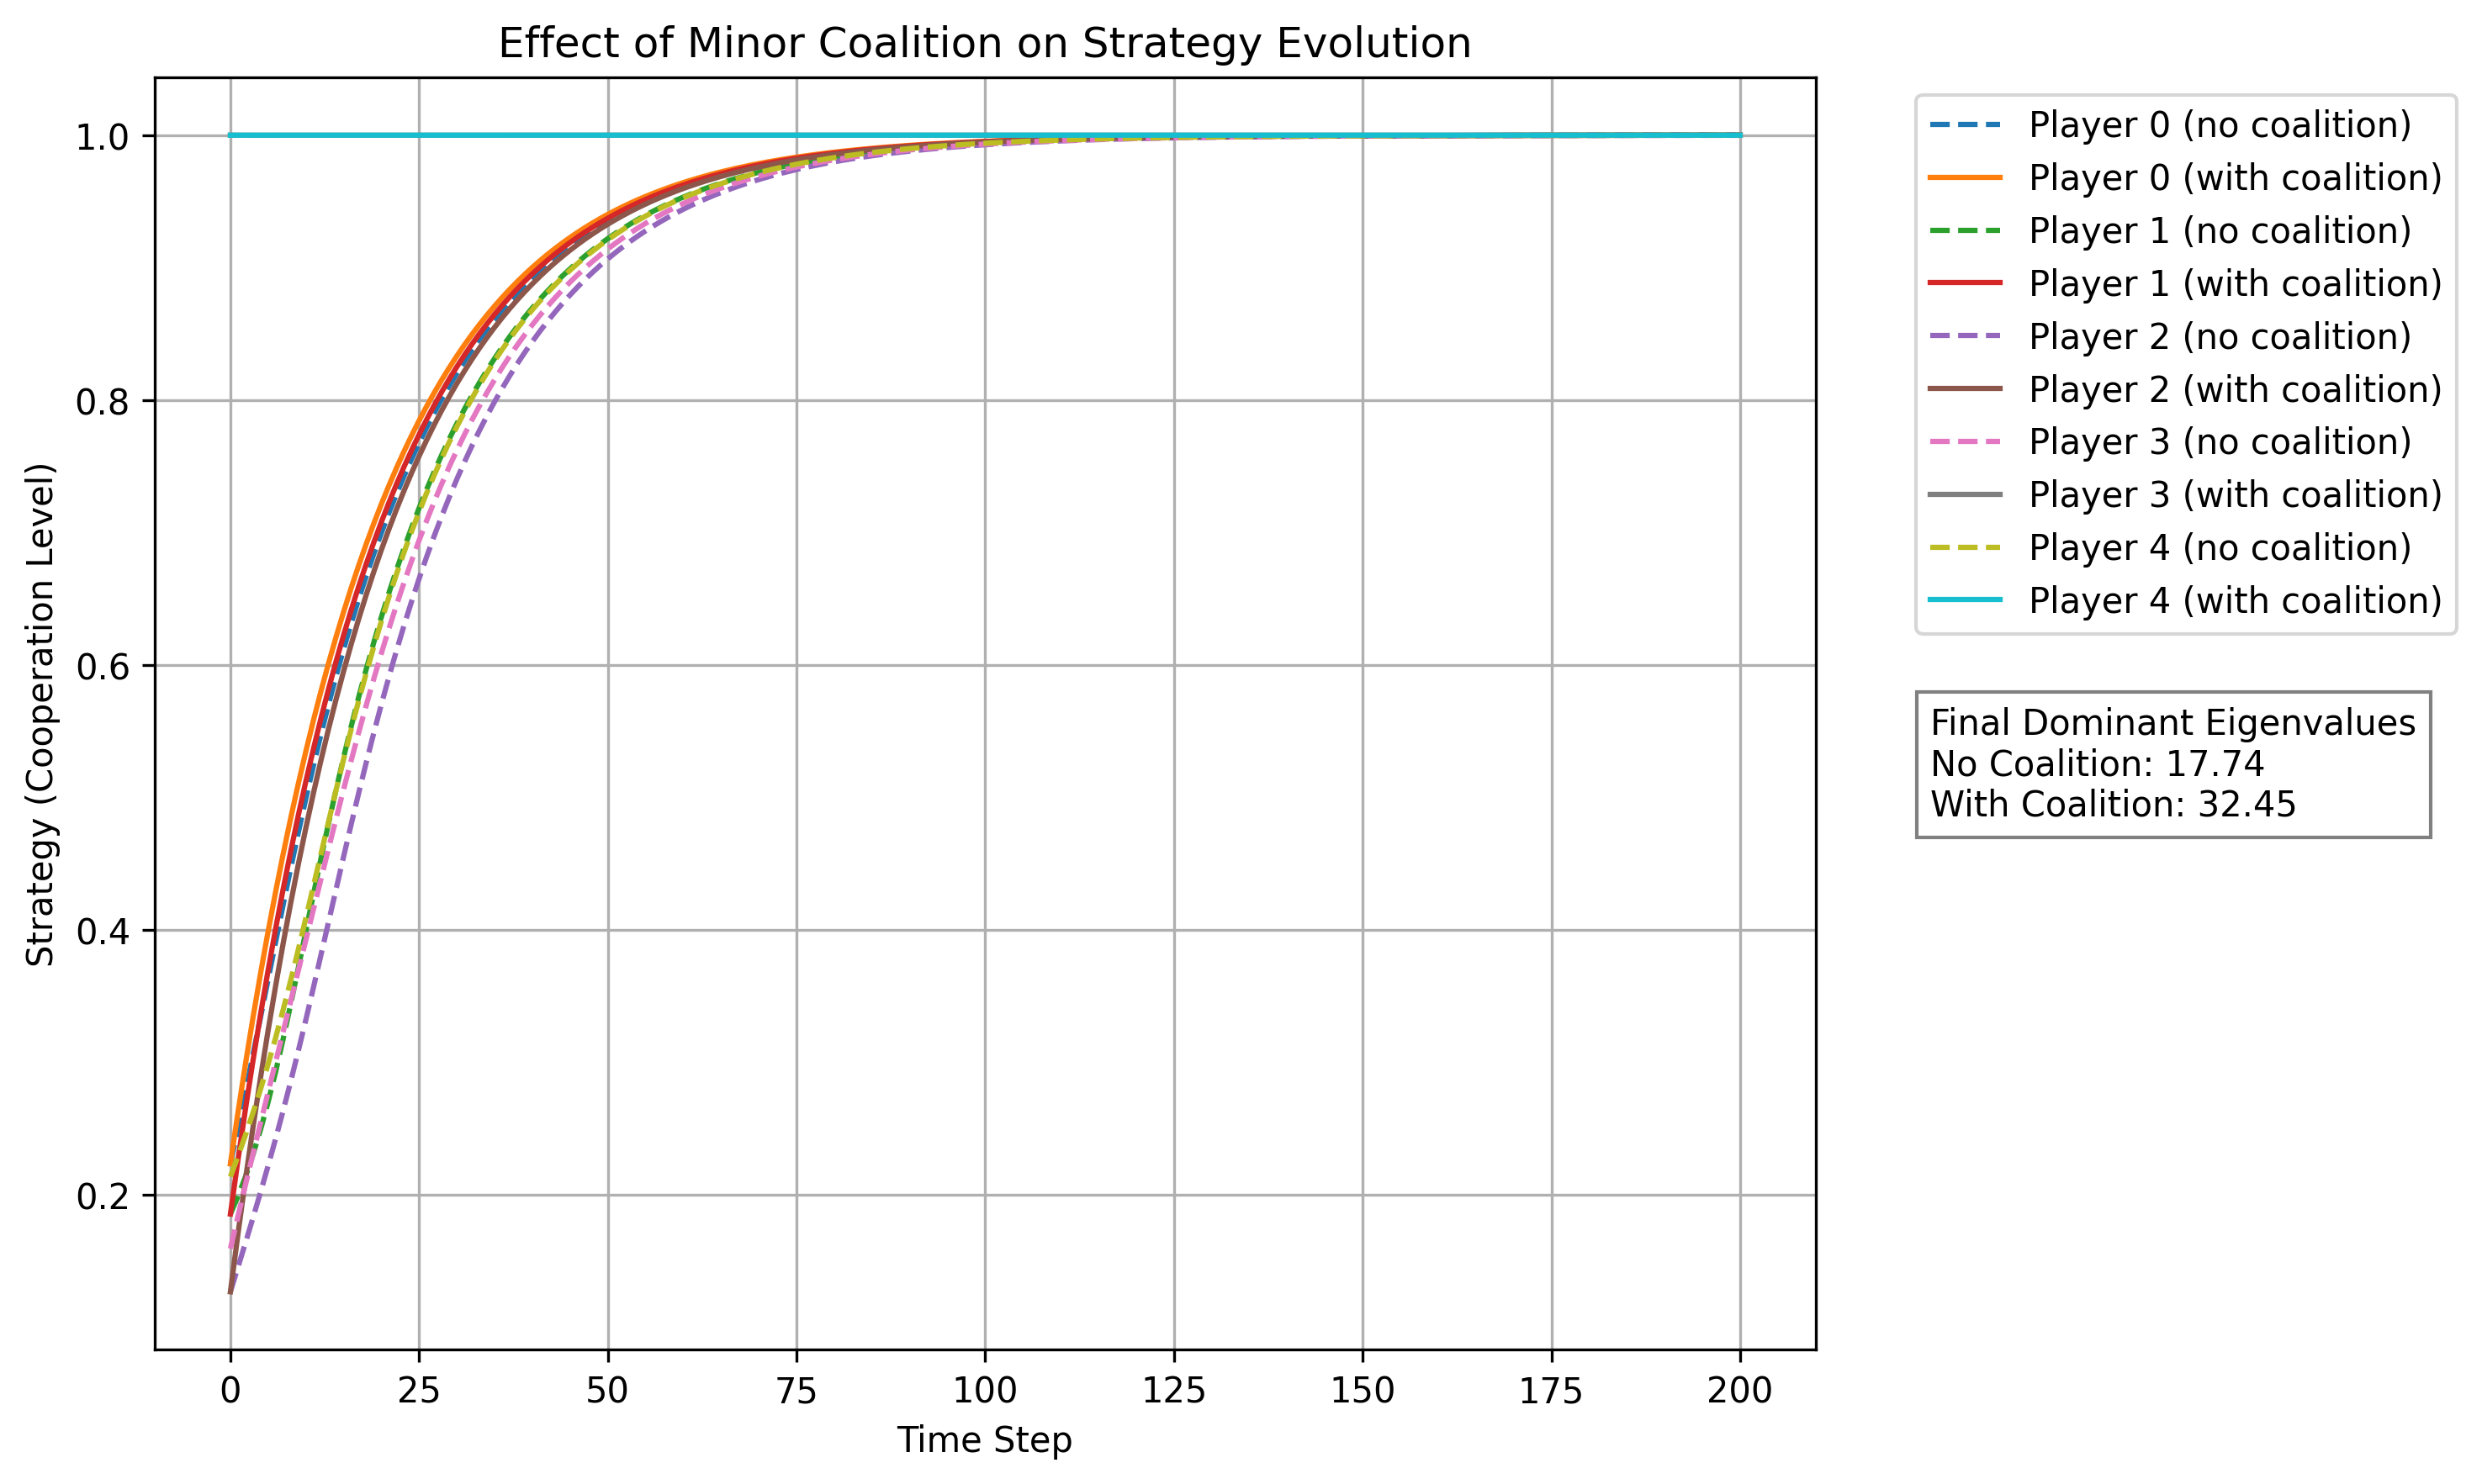
\includegraphics[width=0.85\textwidth]{figures/figure_coalition_effect.png}
	\caption{
		Strategy evolution over time for five players in a tensor-based climate cooperation game. 
		Dashed lines represent strategy levels without any coalition influence, while solid lines show the effect of a minor coalition (players 3 and 4) committed to full cooperation and amplified influence.
		The system's dominant eigenvalue — a proxy for its susceptibility to tipping — increases from 17.74 to 32.45 when the coalition is activated, indicating a shift to a more cooperation-prone regime.
	}
	\label{fig:coalition_tipping}
\end{figure}

\subsection{Scaling Coalition Size in a Larger System}

We extend the simulation to a ten-player system ($N=10$) with three major players (0--2) and seven minor players (3--9). We simulate a sweep across increasing coalition sizes drawn from the minor players. For each coalition size $k$, the selected $k$ players are forced into full cooperation and their influence is amplified. We track both:
\begin{enumerate}
	\item the dominant eigenvalue of the influence matrix at equilibrium;
	\item the average final cooperation level across all players.
\end{enumerate}

\begin{figure}[htbp]
	\centering
	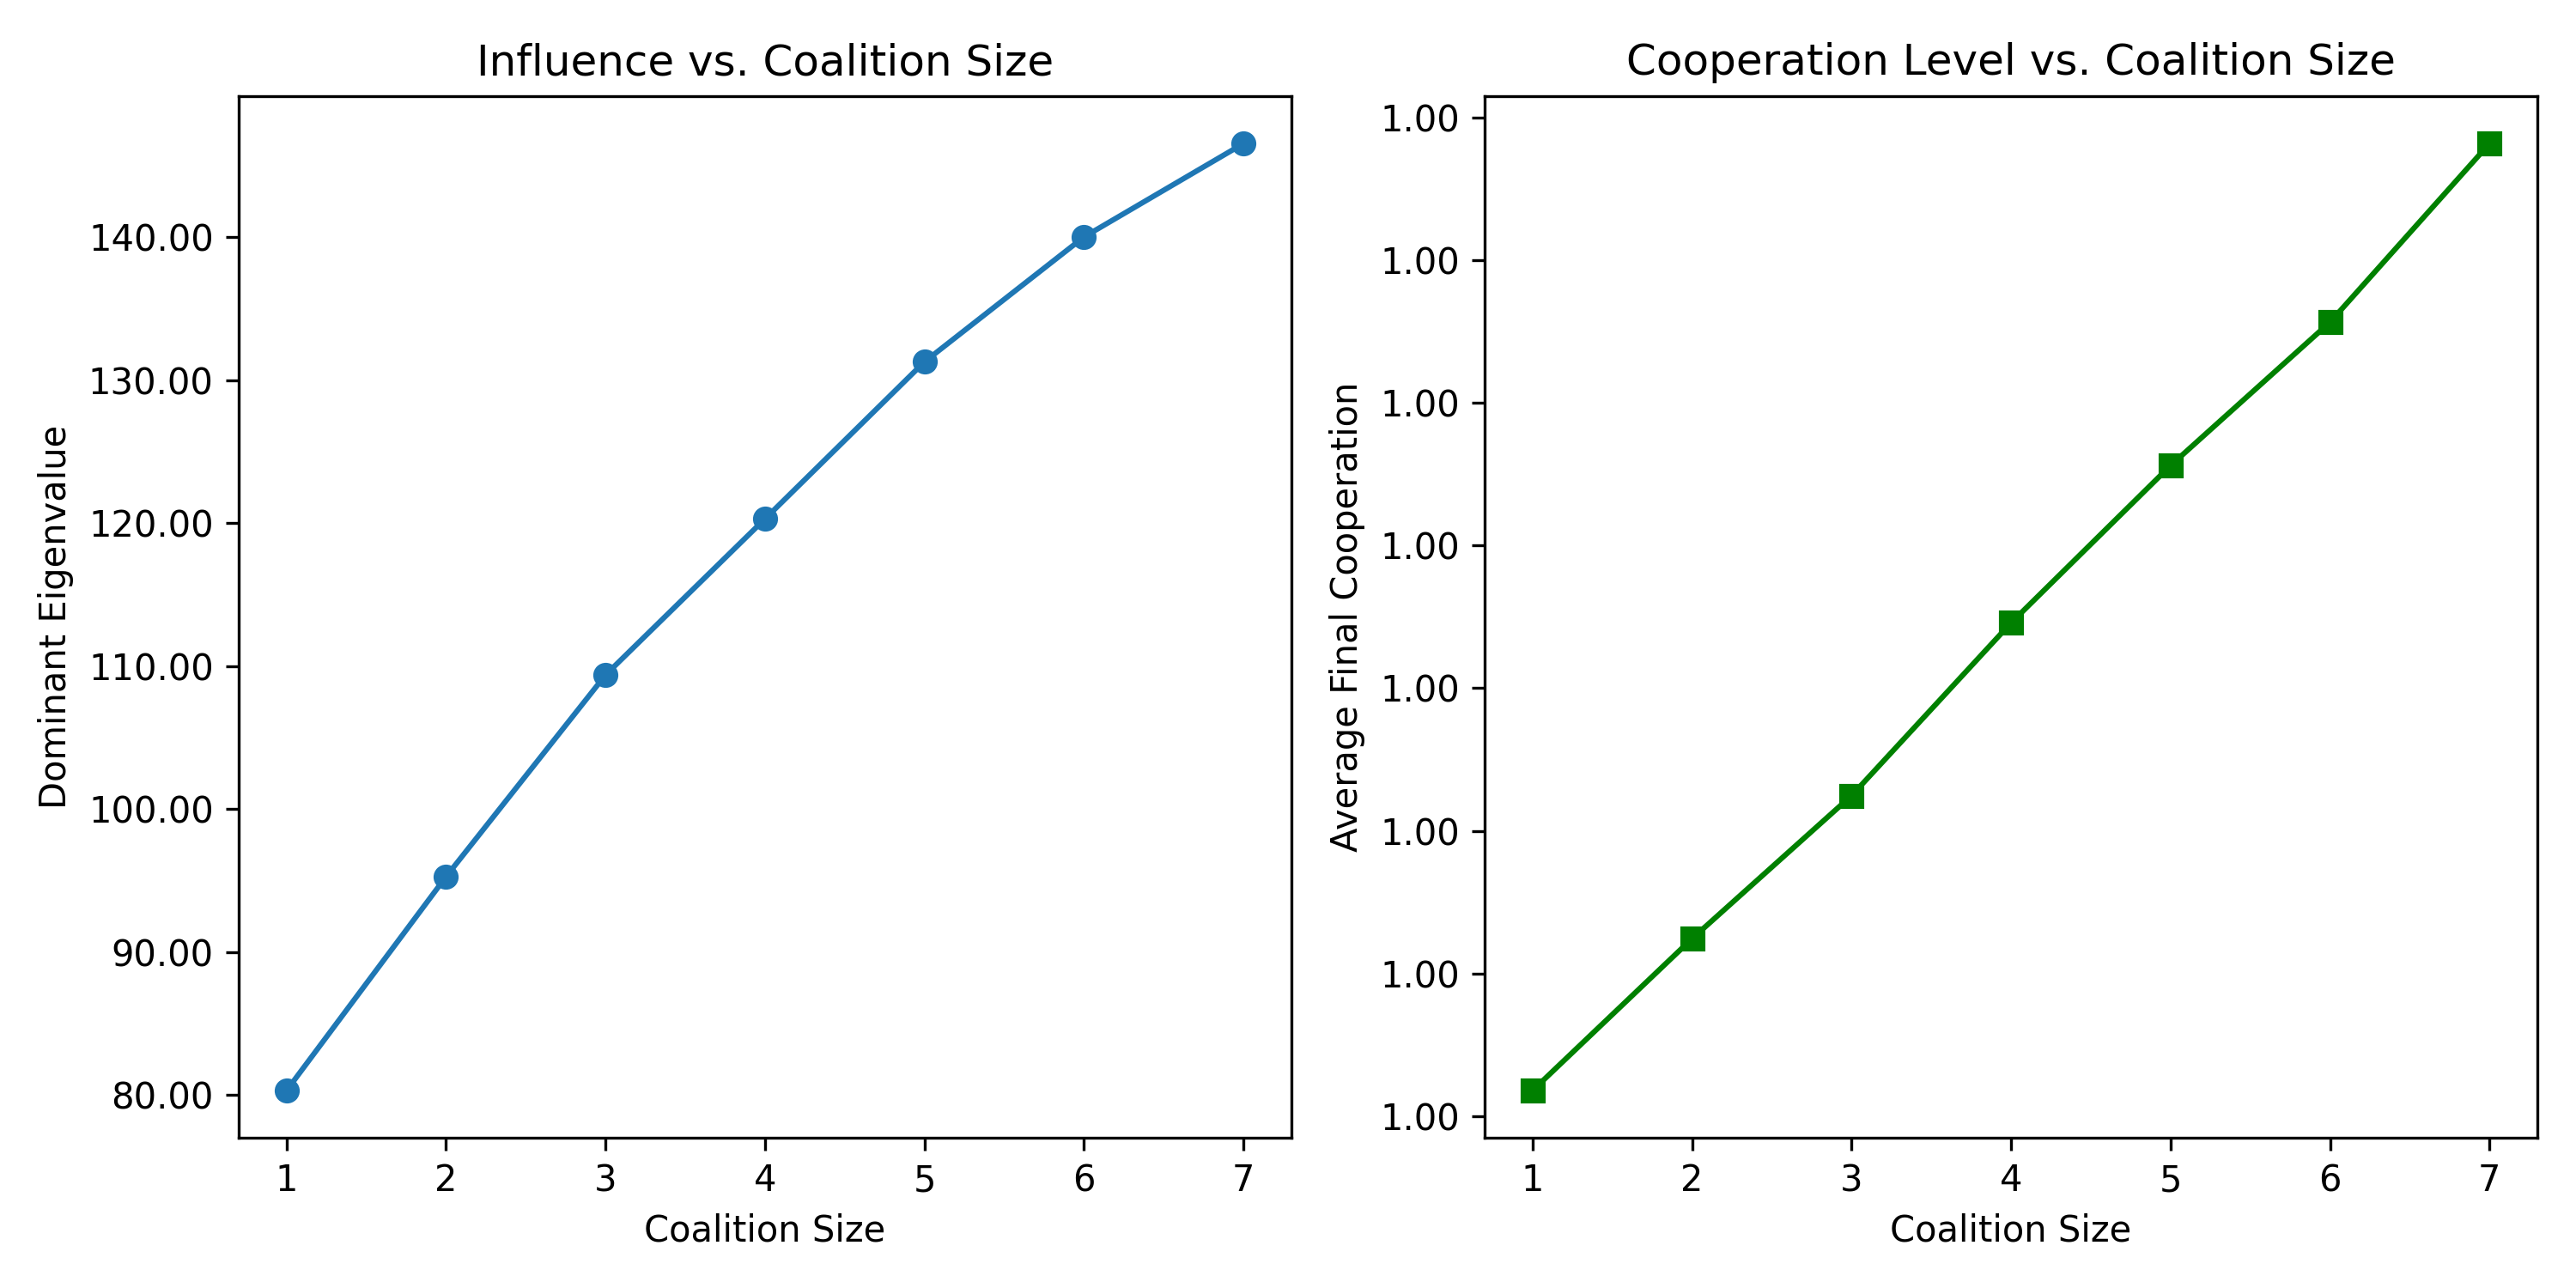
\includegraphics[width=0.95\textwidth]{figures/coalition_sweep_plot.png}
	\caption{
		Influence vs. coalition size experiment. 
		As minor players are incrementally added to a fully cooperating coalition, the dominant eigenvalue of the influence tensor (left) increases non-linearly, indicating higher system susceptibility to tipping.
		Simultaneously, the average final cooperation level (right) rises across all players, showing that even small coalitions can induce broader alignment in strategy.
	}
	\label{fig:coalition_sweep}
\end{figure}

\subsection{Minimum Tipping Coalition and Efficiency}

We define a tipping coalition as any group whose activation causes the dominant eigenvalue $\lambda_{\max}$ to cross a threshold $\lambda_{\text{crit}} = 30$. We exhaustively search all subsets of minor players (3–9), simulate each case, and compute both tipping and per-member efficiency:
\[
\varepsilon(C) = \frac{\lambda_{\max}(C) - \lambda_0}{|C|}
\]

\begin{figure}[htbp]
	\centering
	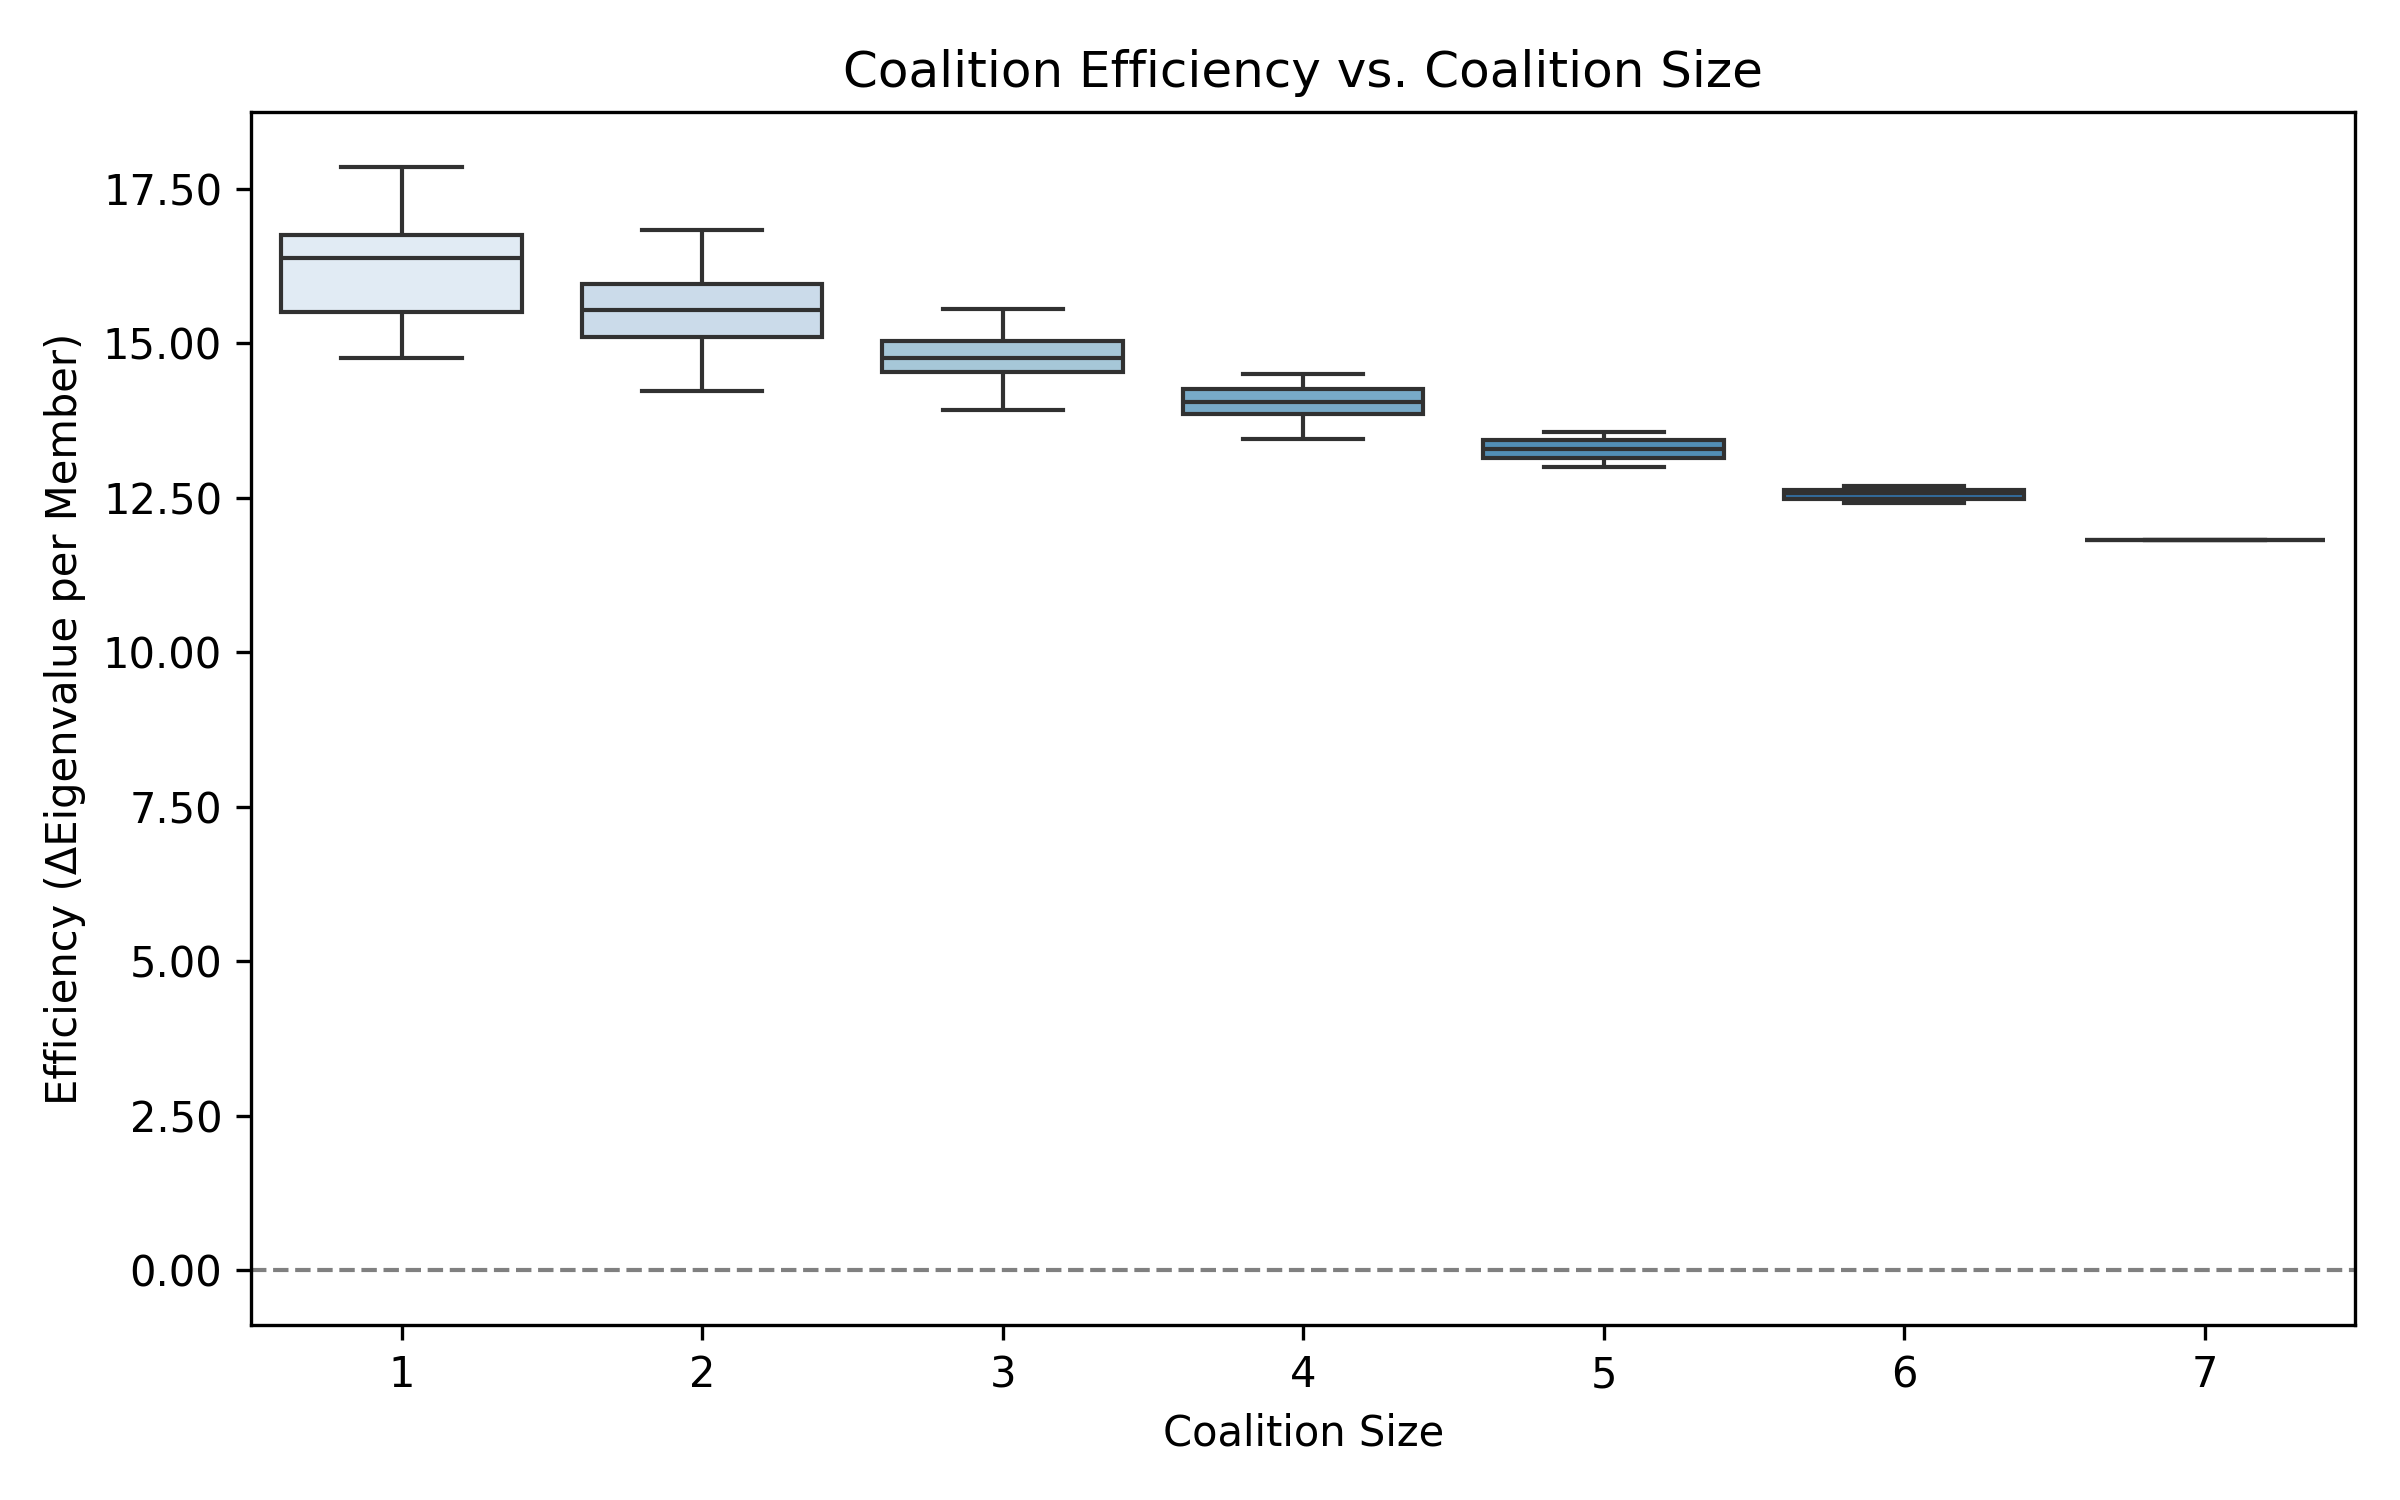
\includegraphics[width=0.8\textwidth]{figures/coalition_efficiency_plot.png}
	\caption{
		Distribution of coalition efficiency scores $\varepsilon(C)$ across coalition sizes. Efficiency is defined as the eigenvalue gain per cooperating member. Smaller coalitions are often more efficient, demonstrating that tipping potential depends more on player influence and position than coalition size alone.
	}
	\label{fig:coalition_efficiency}
\end{figure}

We find that certain small coalitions — even of size 1 — can tip the system if the player is sufficiently influential. This validates that strategic placement and influence structure outweigh raw coalition size.

\subsection{Power Indices and Network Centrality}

To evaluate structural influence and pivotality in coalition dynamics, we compute both game-theoretic and network-based metrics for each player.

We estimate each player’s \textit{Shapley} and \textit{Banzhaf} indices using Monte Carlo sampling over random coalition formations. The Shapley index reflects a player's expected marginal contribution averaged over all possible coalition permutations. The Banzhaf index counts how frequently a player is decisive in turning a losing coalition into a winning one. Both are classical power indices in cooperative game theory~\cite{shapley1953value, banzhaf1965weighted}. These indices represent the likelihood that a player is critical to the success of a coalition. High-index players frequently shift coalition outcomes and thus represent valuable candidates for minimal tipping coalitions.

Additionally, we construct a synthetic network simulating trade or geopolitical ties and compute standard centrality measures: \textit{betweenness centrality} (a proxy for broker power) and \textit{eigenvector centrality} (a recursive measure of influence proximity). Players scoring highly on these centrality metrics are structurally positioned to propagate influence.

\begin{figure}[htbp]
	\centering
	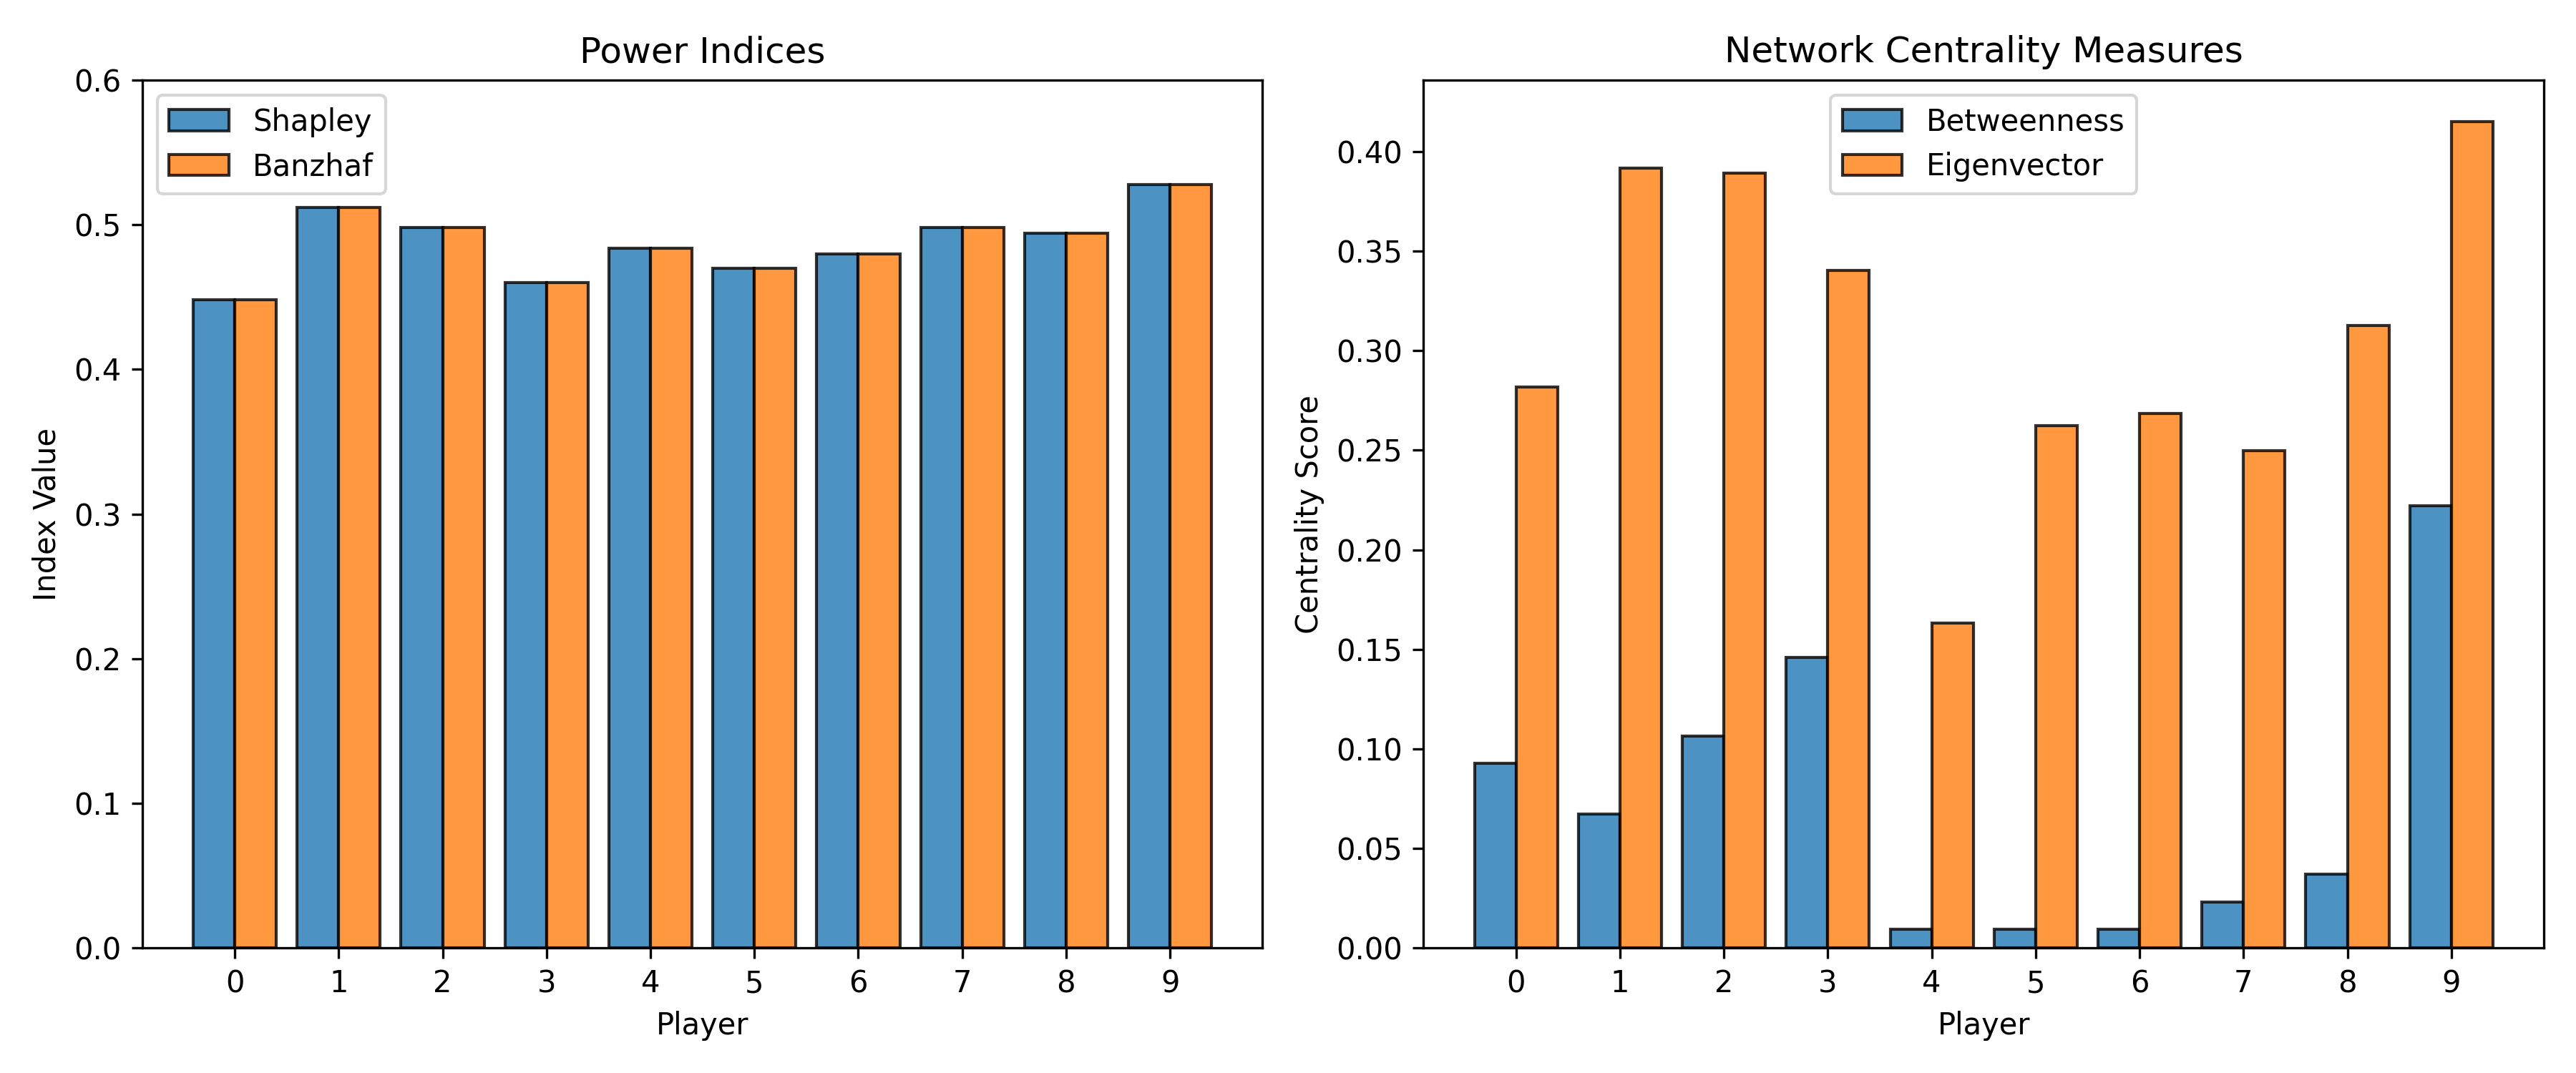
\includegraphics[width=0.95\textwidth]{figures/figure_power_centrality.png}
	\caption{
		Power and centrality analysis of players in a simulated climate game. 
		Left: Shapley and Banzhaf indices show which players are frequently pivotal in coalitional outcomes.
		Right: Betweenness and eigenvector centrality from a synthetic influence network. Structurally central players have higher strategic leverage.
	}
	\label{fig:power_centrality}
\end{figure}

Figure~\ref{fig:power_centrality} confirms that players with high pivotality often overlap with those holding structural centrality in the interaction network. High scores on both metrics jointly flag actors whose removal would most reduce coalition tipping potential.


\subsection{Greedy Search for Minimal Tipping Coalitions}

We implement a greedy search heuristic that iteratively adds players to a coalition based on marginal gains in the system’s dominant eigenvalue. Starting with an empty coalition, each iteration selects the player who produces the largest incremental increase in simulated system responsiveness, terminating when the eigenvalue crosses a tipping threshold $\lambda_{\text{crit}} = 30$.

This method provides a computationally efficient alternative to exhaustive enumeration and often identifies near-minimal tipping coalitions that align with insights from power indices and coalition efficiency metrics.

\begin{figure}[htbp]
	\centering
	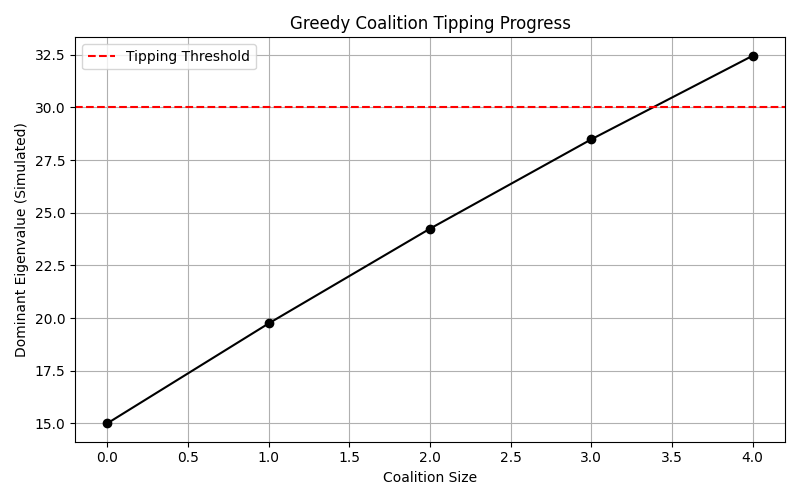
\includegraphics[width=0.8\textwidth]{figures/figure_greedy_tipping.png}
	\caption{
		Simulated dominant eigenvalue as a function of coalition size, using a greedy heuristic. Players are added one at a time based on marginal eigenvalue gain. The system crosses the tipping threshold after only four players are added, highlighting the strategic leverage of a small, targeted group.
	}
	\label{fig:greedy_tipping}
\end{figure}

\vspace{0.5em}

The implementation used to generate Figure~\ref{fig:greedy_tipping} is available at:
[details withheld for double-anonymous review]


\subsection{Reinforcement Learning for Coalition Formation}

We train a reinforcement learning agent using the REINFORCE algorithm to learn coalition formation strategies. The policy network outputs inclusion probabilities for each nation, and coalitions are sampled from these distributions at each training step. Rewards are computed based on system-wide cooperation, tipping behaviour, and coalition size constraints.

Three reward models are tested:

\begin{itemize}
	\item \textbf{Raw Reward:} Favours maximum cooperation — leads to full coalitions.
	\item \textbf{Penalised Reward:} Subtracts size-based costs; requires careful tuning.
	\item \textbf{Threshold-Based Reward:} Rewards tipping within a size cap (e.g., $\leq 5$).
\end{itemize}

Training reveals that:
\begin{itemize}
	\item Raw reward leads to convergence on all 10 players.
	\item Penalised reward leads to mid-sized, efficient coalitions when properly tuned.
	\item Threshold reward reliably finds minimal tipping sets (e.g., 3–4 members).
\end{itemize}

We experiment with various penalty structures:
\[
\text{reward} = \text{gain} - \alpha \cdot |C|^2
\]
to control coalition bloat and prioritise strategic leverage over size. In experiments, $\alpha = 0.1$ is used for the penalised condition.

\begin{figure}[htbp]
	\centering
	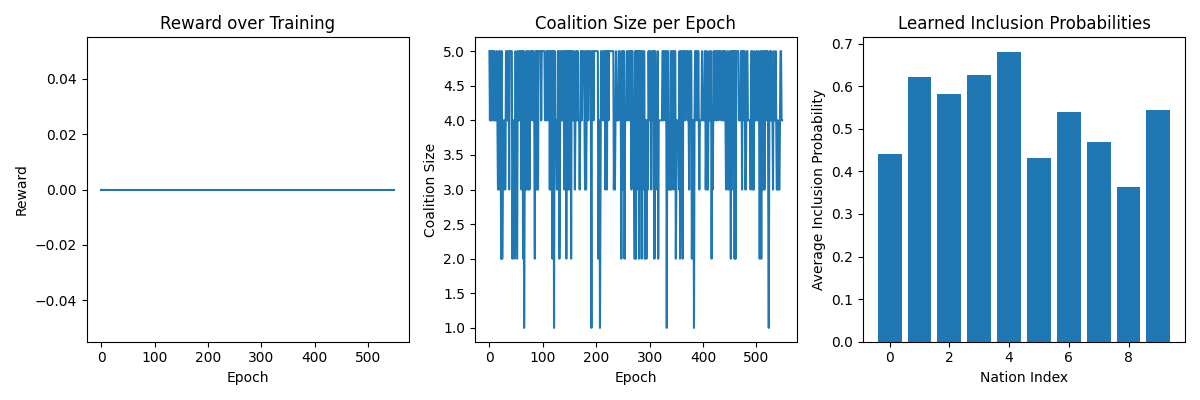
\includegraphics[width=0.95\textwidth]{figures/figure_rl_training_summary.png}
	\caption{
		RL training metrics under the threshold-based reward function. 
		\textbf{Left:} reward over epochs shows sparse but stable learning. 
		\textbf{Middle:} coalition size converges to 3–5 players.
		\textbf{Right:} average inclusion probabilities for each nation over training, highlighting which actors are consistently selected.
	}
	\label{fig:rl_training_summary}
\end{figure}

Figure~\ref{fig:rl_training_summary} shows learning dynamics over time. Despite sparse rewards, the agent successfully converges to a compact, high-impact coalition. The threshold reward variant produces the most compact and interpretable coalitions; raw reward leads to over-inclusion and penalised reward requires careful tuning of $\alpha$.

Full source code for this experiment is available at:  
[details withheld for double-anonymous review]



\section{Clustering Countries by Treaty Participation}
\label{sec:clustering}

To investigate the strategic alignment of countries within the context of international environmental agreements, we analyse the IEA ratification dataset~\cite{bellelli2021iea}, which provides comprehensive data on participation in 263 multilateral treaties from 1950 to 2017. We construct a binary country--treaty matrix and compute pairwise similarity between countries based on shared ratification profiles.

We apply hierarchical clustering using cosine similarity and Ward linkage to partition countries into eight primary clusters. Each cluster is labelled descriptively by its dominant UNSD sub-region (e.g., \textit{Northern Africa(6) + 4 more}), providing a high-level summary of geopolitical alignment and regional proximity.

Figure~\ref{fig:cluster_network} presents the resulting cluster-to-cluster similarity network. Edges indicate strong cosine similarity (threshold $\geq 0.5$) between average treaty profiles of different clusters, and labels summarise the dominant subregion and diversity of membership.

\begin{figure}[htbp]
	\centering
	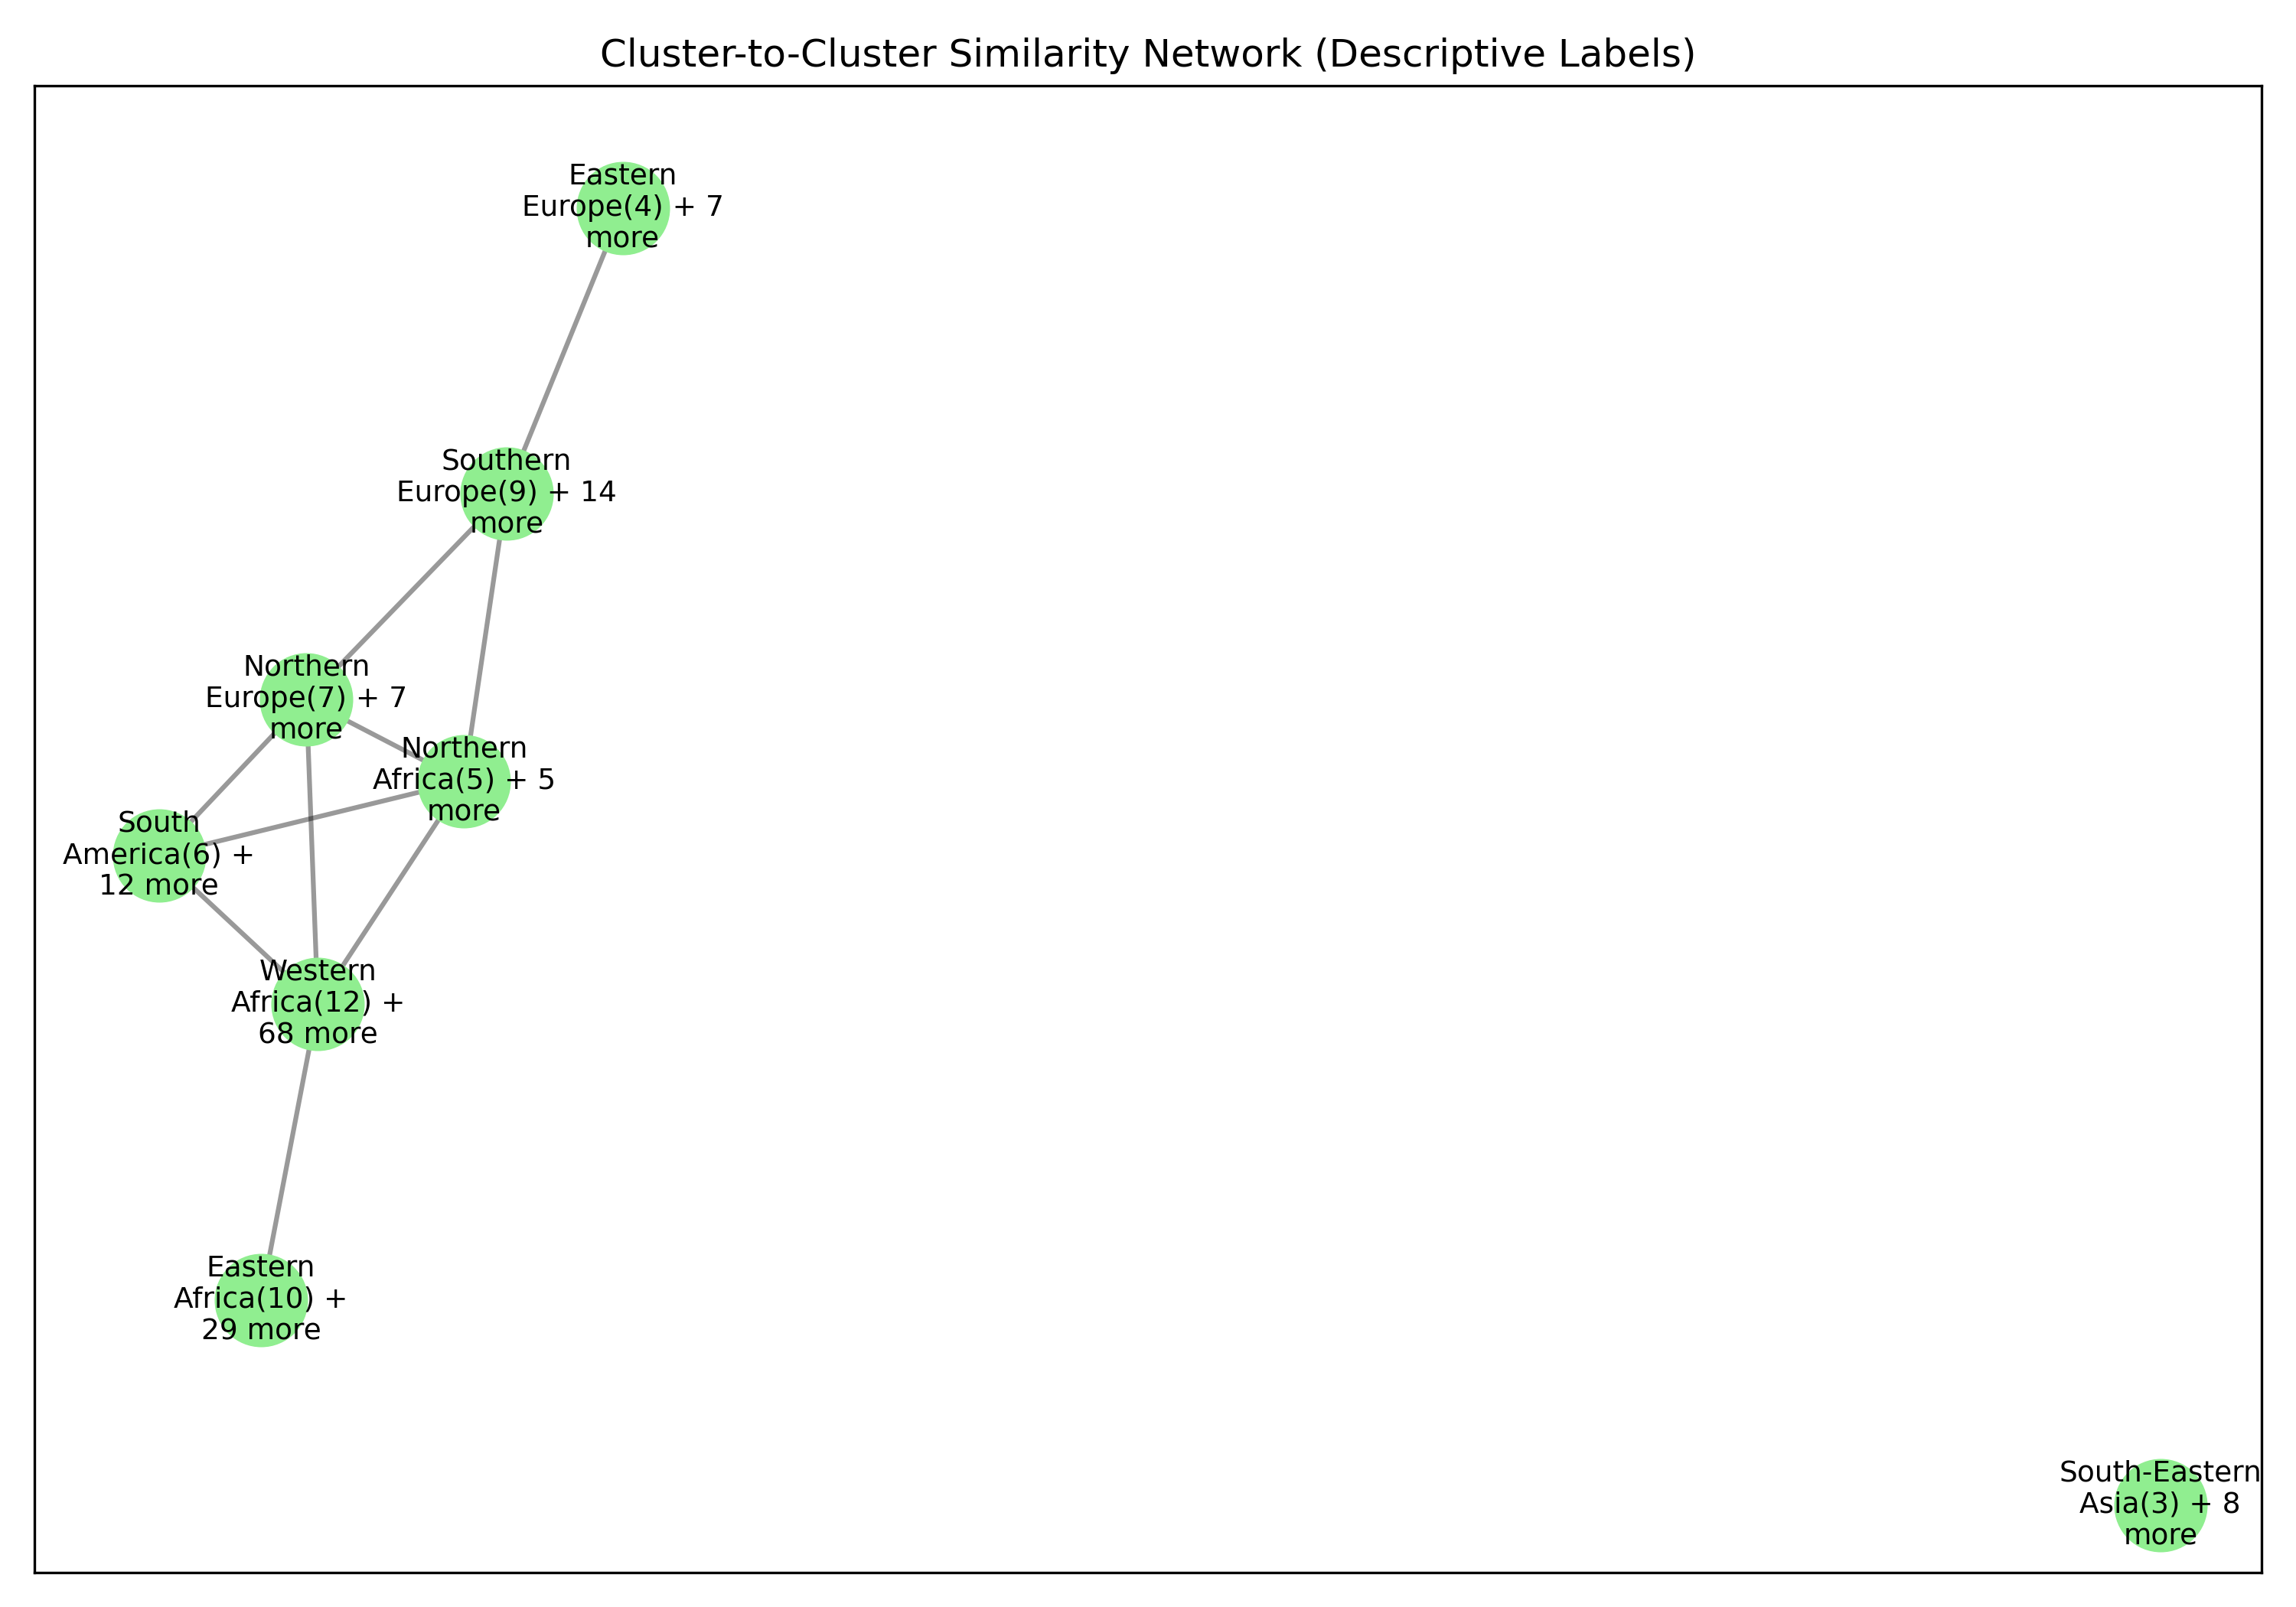
\includegraphics[width=0.9\textwidth]{figures/figure_pca_country_similarity.png}
	\caption{
		Similarity network between clusters of countries based on co-ratification of international environmental treaties. Nodes represent clusters labelled by their dominant subregion. Edges reflect strong average cosine similarity between clusters, suggesting historical alignment or shared priorities.
	}
	\label{fig:cluster_network}
\end{figure}

Within each cluster, we further examine strategic similarity using PCA projections. These visualisations (see supplementary figures) provide insight into intra-cluster cohesion, while dendrograms reveal potential substructures. Cluster 5 contains a disproportionately large number of countries, and its dendrogram suggests at least three cohesive sub-clusters. A more detailed sub-clustering of such large groups may help refine our understanding of coalition boundaries and is proposed for future work.

\subsection*{Strategic Motivation for Minor Player Alliance Search}

Our primary motivation in identifying these clusters is to support the discovery of new, strategically interesting alliances among \emph{minor players}. Within-cluster alignments are likely to reflect existing blocs, formal or informal (e.g., shared regional institutions, UN voting patterns). These are not only intuitive but likely already explored diplomatically.

However, coalitions that span multiple clusters may be less obvious—and more valuable. We hypothesise that \textbf{cross-cluster alliances among minor players} can form unexpected but influential coalitions with high leverage in shifting larger players' strategies. The clustering analysis provides a principled basis for scanning such cross-community combinations.

\subsection{Exhaustive Search for Minor-Player Tipping Coalitions}
\label{sec:minor_coalitions}

To operationalise our tipping-point model on real data, we implemented an exhaustive search over potential coalitions of \textit{minor players}, defined here as countries not in the G20. For each coalition of size 2 to 4, we computed a composite tipping score that combines three criteria:

\begin{enumerate}
	\item \textbf{Alignment}: the mean pairwise cosine similarity of treaty ratification profiles within the coalition.
	\item \textbf{Influence spread}: the total treaty co-ratification overlap from coalition members to all non-members, measured as $\sum_{i \in C,\, j \notin C} \mathbf{x}_i \cdot \mathbf{x}_j$ where $\mathbf{x}_i$ is the binary treaty vector of country $i$. This metric counts aggregate shared treaty commitments across the coalition boundary and is the same quantity used in the reinforcement learning reward function (Section~\ref{sec:results_rl}).
	\item \textbf{Cluster diversity}: the number of distinct treaty-participation clusters represented in the coalition.
\end{enumerate}

Each coalition \( C \) received a score defined as:
\[
\text{TippingScore}(C) = \text{Alignment}(C) \times \text{InfluenceSpread}(C) \times \text{ClusterDiversity}(C)
\]

\paragraph{Computational Performance.}
Although conceptually simple, this approach scales combinatorially. Given \( n \) minor players, there are:

\[
\sum_{k=2}^4 \binom{n}{k} = O(n^4)
\]

coalitions to evaluate. With \( n = 175 \) minor players in the corrected pipeline, the number of 2--4 member coalitions is:
\[
\binom{175}{2} + \binom{175}{3} + \binom{175}{4} = 15{,}225 + 877{,}975 + 37{,}752{,}925 \approx 38.6 \text{ million}
\]
The 2- and 3-member searches complete in under one minute. The 4-member search completes in approximately 30 minutes. Extending to 5-member coalitions would add a further 1.3~billion combinations and was not attempted.

\paragraph{Scalability.}
For larger coalition sizes, exhaustive enumeration becomes intractable. We address this in subsequent sections using greedy forward selection and reinforcement learning, both of which discover high-scoring coalitions without full enumeration.

\subsection{Empirical Calibration of Tipping Thresholds}
\label{sec:empirical_tipping_threshold}

In Section~\ref{sec:minor_coalitions}, we defined a tipping coalition as one that induces a qualitative shift in the strategic equilibrium through amplified internal alignment and influence spread. Although this is analytically expressed through tensor bifurcation behaviour, its empirical counterpart can be approximated via our coalition scoring framework.

To this end, we computed a composite score for all 2–3 member coalitions of minor (non-G20) countries:
\[
\text{TippingScore}(C) = \text{Alignment}(C) \times \text{InfluenceSpread}(C) \times \text{ClusterDiversity}(C)
\]
where:
\begin{itemize}
	\item \textbf{Alignment(C)} is the mean pairwise cosine similarity within the coalition,
	\item \textbf{InfluenceSpread(C)} is the total treaty co-ratification overlap from coalition members to all non-members ($\sum_{i \in C, j \notin C} \mathbf{x}_i \cdot \mathbf{x}_j$),
	\item \textbf{ClusterDiversity(C)} counts the number of distinct ratification clusters represented in \( C \).
\end{itemize}

\paragraph{Distribution Analysis.}
As shown in Figure~\ref{fig:score_distribution}, the tipping scores form a positively skewed distribution with a long upper tail. The mean score across all 893{,}200 two- and three-member coalitions is 14{,}190 with a standard deviation of 4{,}678. The top 1\% of coalitions exceed a score of 24{,}599, reaching up to 33{,}527.

\begin{figure}[htbp]
	\centering
	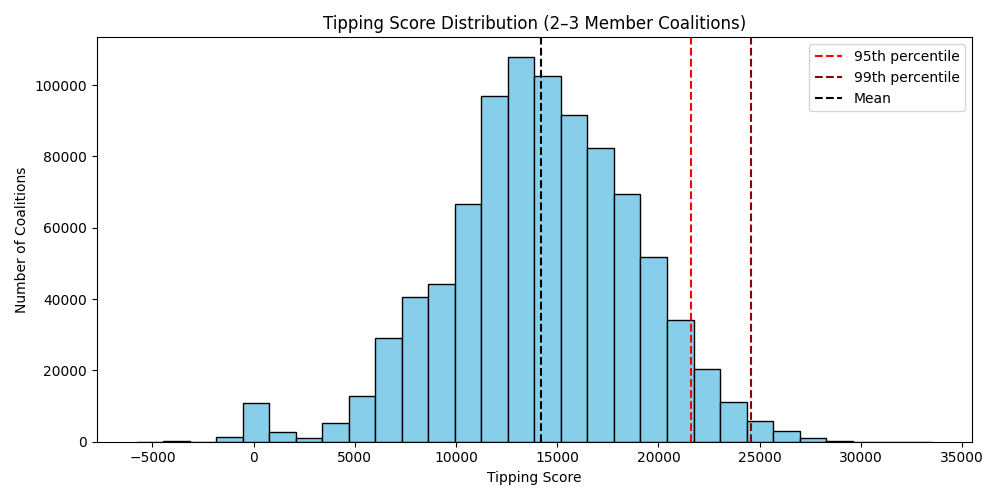
\includegraphics[width=0.85\textwidth]{figures/score_distribution_2to3.png}
	\caption{
		Distribution of tipping scores across all 2–3 member minor-player coalitions. 
		The 95th and 99th percentile thresholds are marked in red, indicating rare, high-impact alignments.
	}
	\label{fig:score_distribution}
\end{figure}

\paragraph{Tipping Threshold Definition.}
We designate the 99th percentile value (24{,}599) as a data-driven tipping threshold. This is an empirical criterion, not a derivation of the analytical bifurcation threshold $\lambda_c$ from Section~\ref{sec:math}: unlike $\lambda_c$, which is defined by the saddle-node structure of Equation~\eqref{eq:dynamics}, the p99 threshold is defined post-hoc from the observed score distribution. It serves as an operational filter for identifying statistically exceptional coalitions --- those in the upper 1\% of strategic cohesion and influence reach --- and provides a quantitative analogue to the qualitative concept of a tipping coalition introduced in Section~\ref{sec:math}. Future work (Section~\ref{sec:future}) could calibrate $\lambda_c$ against historical negotiation outcomes to replace this empirical proxy with a theoretically-grounded criterion.

\paragraph{Examples.}
One illustrative coalition exceeding this threshold is:
\[
\texttt{(Spain, Croatia, Morocco)}
\]
with a tipping score of 33{,}527. These three countries span Southern Europe and North Africa, exhibit high pairwise treaty alignment, and provide strong cross-cluster influence reach, making them a plausible catalytic grouping under the tipping framework.

The full list of top-scoring coalitions is available in the supplementary dataset (compressed):
\begin{quote}
	[details withheld for double-anonymous review]
\end{quote}

This empirical framework provides a quantitative, justifiable method to surface candidate alliances for international coordination.

\subsection{Fast Greedy Search for Tipping Coalitions}
\label{sec:greedy_coalitions}

Due to the combinatorial explosion of coalition configurations among minor players, we implemented a fast greedy forward-selection algorithm to identify high-scoring coalitions of up to six members. At each step, a new player is added if doing so increases the composite tipping score, subject to a cluster diversity constraint: no single cluster may represent more than half the coalition.

\paragraph{Method.}
To improve efficiency, we pre-compute:
\begin{itemize}
	\item All pairwise cosine similarities between countries;
	\item Aggregate influence spread from each minor player to all others.
\end{itemize}

This allows coalition scores to be calculated in constant time using cached values.

\paragraph{Results.}
The distribution of coalition tipping scores is shown in Figure~\ref{fig:greedy_score_hist}. The top-scoring coalition identified by the greedy search is \{Mauritius, Jamaica, Ireland, Greece, Tunisia, Uruguay\} with a tipping score of 105{,}353, substantially higher than typical 2--3 member coalitions due to the larger size, high internal alignment, and influence reach across 6 of 8 treaty clusters. The majority of successful coalitions span multiple clusters, meeting our criteria for potential systemic influence.

\paragraph{Comparison note.}
The greedy algorithm optimises raw TippingScore (Equation~\ref{eq:tipping_score}) without per-member normalisation or vulnerability weighting. The reinforcement learning agent in Section~\ref{sec:results_realdata} optimises a different objective --- TippingScore$\,\times\,(1 + 0.5\,\bar{v}_C)\,/\,|C|$ --- which rewards per-member efficiency and vulnerability representation. Scores from the two methods are therefore on different scales and should not be compared directly. To recover a comparable base TippingScore for an RL coalition, multiply the reported RL score by $|C| / (1 + 0.5\,\bar{v}_C)$.

\begin{figure}[htbp]
	\centering
	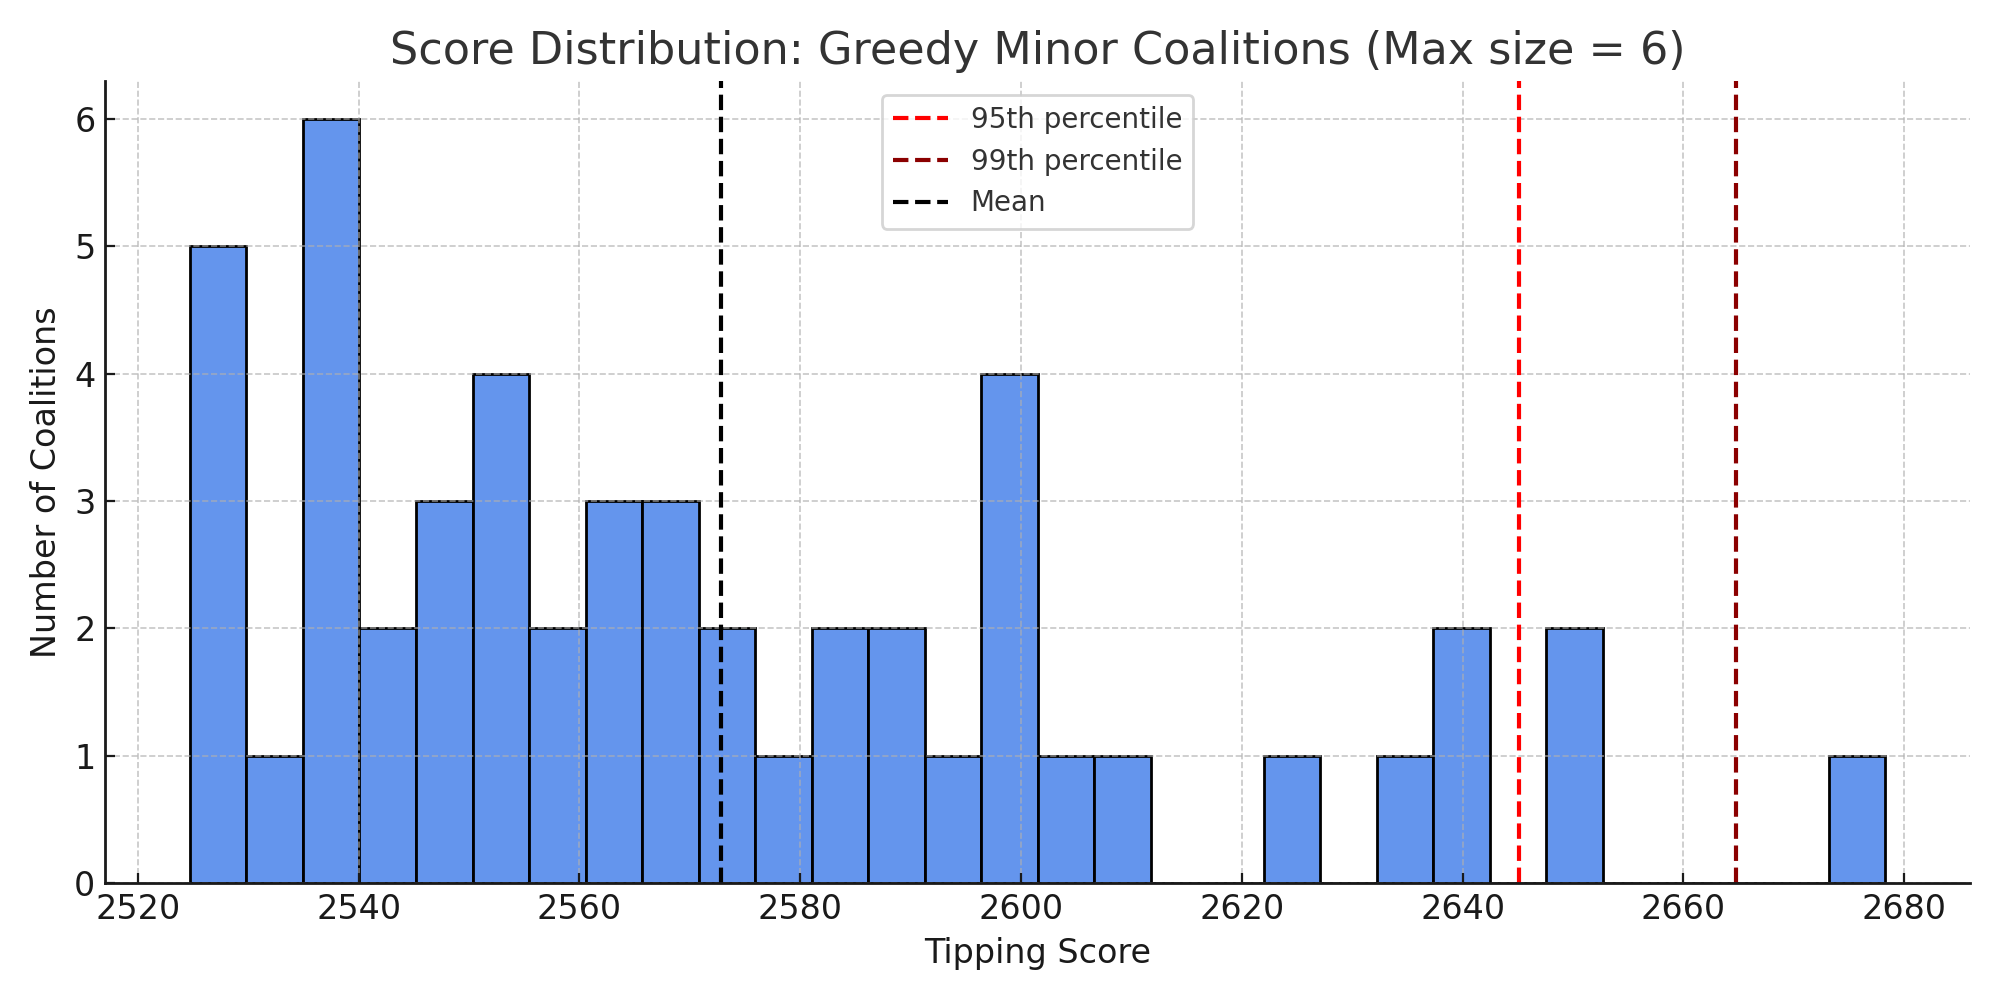
\includegraphics[width=0.85\textwidth]{figures/greedy_score_distribution.png}
	\caption{Distribution of tipping scores for top minor-player coalitions discovered using greedy forward-selection.}
	\label{fig:greedy_score_hist}
\end{figure}

\paragraph{Structural Interpretation.}
Figure~\ref{fig:greedy_coalition_network} presents a network of coalition memberships, where edges indicate co-occurrence in high-scoring coalitions. The structure reveals recurring strategic partnerships and frequently co-occurring actor pairings.

\begin{figure}[htbp]
	\centering
	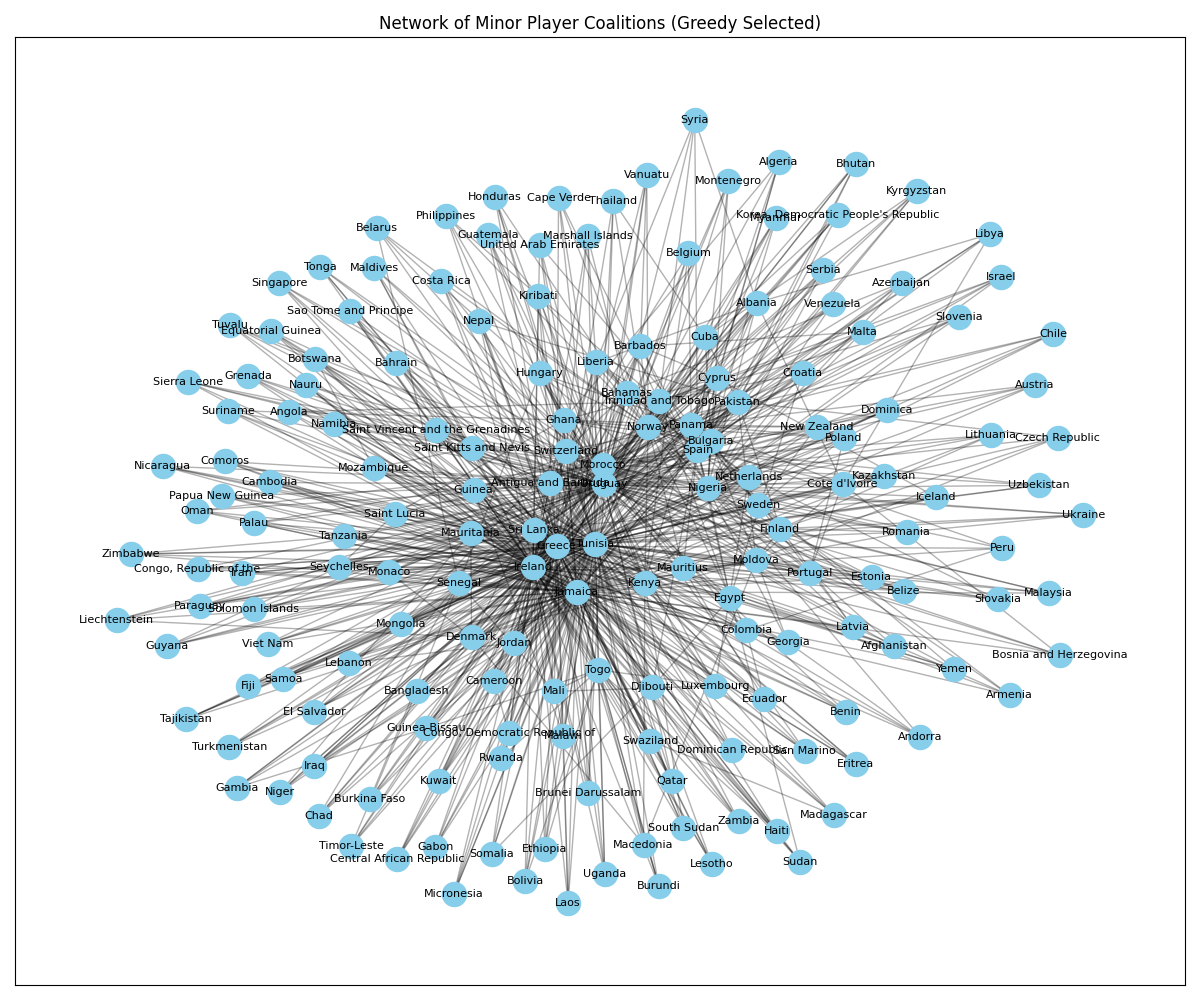
\includegraphics[width=0.85\textwidth]{figures/greedy_minor_coalition_network.png}
	\caption{Network of minor players frequently co-occurring in high-scoring coalitions under the greedy search strategy.}
	\label{fig:greedy_coalition_network}
\end{figure}

\subsection{Empirical Validation Against Real-World Coalitions}
\label{sec:empirical_validation}

To assess the empirical plausibility of the coalitions identified by our model, we compared our top-ranked minor-player coalitions against known international climate groupings:

\begin{itemize}
	\item \textbf{High Ambition Coalition (HAC)}~\cite{hochstetler2019ambition} — a diplomatic bloc that successfully pushed for the 1.5°C temperature goal in the Paris Agreement;
	\item \textbf{Alliance of Small Island States (AOSIS)}~\cite{aosis2023} — a long-standing coalition of climate-vulnerable island nations;
	\item \textbf{Fossil Fuel Non-Proliferation Treaty (FF-NPT) Initiative}~\cite{ffnpt2024} — a recent campaign led by vulnerable nations seeking to phase out fossil fuel production.
\end{itemize}

We found that several of our model-identified coalitions contain members from these influential real-world initiatives. For example, \textit{Jamaica}, \textit{Mauritius}, and \textit{The Bahamas} — all AOSIS members — appear in multiple top-scoring coalitions, as do HAC member states \textit{Ireland}, \textit{Greece}, and \textit{Uruguay} (see Table~\ref{tab:matched_coalitions}). All 164 unique greedy-discovered coalitions overlap with at least one of the three initiatives, reflecting the broad geographic reach of HAC and AOSIS membership among non-G20 nations.

\paragraph{Interpretation.}
This overlap supports the model's validity: coalitions flagged as potentially influential by our tipping score framework are not only plausible but often reflect known diplomatic groupings that have, in fact, shaped global policy outcomes.

\paragraph{Limitations and Next Steps.}
Our matching focused only on membership overlap. Future work could extend this by analysing whether these coalitions took joint action within specific negotiation rounds, and whether their emergence preceded shifts in the positions of larger actors.

\begin{table}[htbp]
	\centering
	\scriptsize
	\begin{tabular}{lll}
\toprule
             Initiative &                                  Coalition Members &  Tipping Score \\
\midrule
High Ambition Coalition & Georgia, Maldives, Korea, Republic of, Ireland,... &    2588.970124 \\
High Ambition Coalition & Norway, Bulgaria, Korea, Republic of, Sri Lanka... &    2479.820719 \\
High Ambition Coalition & Maldives, Afghanistan, Papua New Guinea, Algeri... &    2470.885138 \\
High Ambition Coalition & Chile, Pakistan, Paraguay, Tunisia, Ireland, Gr... &    2456.770215 \\
                  AOSIS & Mauritius, Korea, Republic of, Egypt, Greece, I... &    2601.572906 \\
                  AOSIS & Sri Lanka, Papua New Guinea, Korea, Democratic ... &    2601.343474 \\
                  AOSIS & Papua New Guinea, Sri Lanka, Korea, Democratic ... &    2601.343474 \\
                  AOSIS & Algeria, Sri Lanka, Papua New Guinea, Korea, De... &    2601.343474 \\
                  AOSIS & Georgia, Maldives, Korea, Republic of, Ireland,... &    2588.970124 \\
     Fossil Fuel Treaty & Pakistan, New Zealand, Korea, Democratic People... &    2572.037733 \\
     Fossil Fuel Treaty & Solomon Islands, Papua New Guinea, Sri Lanka, A... &    2493.596324 \\
     Fossil Fuel Treaty &   Swaziland, Togo, Samoa, Tunisia, Ireland, Greece &    2476.830569 \\
     Fossil Fuel Treaty &     Jordan, Sudan, Samoa, Tunisia, Ireland, Greece &    2471.643165 \\
     Fossil Fuel Treaty & Guinea-Bissau, Togo, Samoa, Ireland, Tunisia, G... &    2467.402047 \\
\bottomrule
\end{tabular}

	\caption{Sample of high-scoring minor-player coalitions with overlaps to known real-world initiatives. Full results available at:
		[details withheld for double-anonymous review]}
	\label{tab:matched_coalitions}
\end{table}

\subsection{Reward Strategy Sensitivity Analysis}
\label{sec:rl_reward_strategies}

To evaluate the impact of reward design on reinforcement learning behaviour, we ran a sweep over key parameters using the corrected pipeline ($n = 175$, influence matrix spread metric). Specifically, we varied:
\begin{itemize}
	\item \textbf{Size Cap}: The maximum allowed number of members in a coalition (4, 6, or 8);
	\item \textbf{Penalty $\alpha$}: A size-based reward penalty ($\alpha \in \{0.0, 1.0\}$, applied as $\text{score} / |C|^{\alpha}$);
	\item \textbf{Reward Threshold}: A minimum score filter (none, 2{,}000, or 5{,}000). Thresholds are set relative to the corrected-pipeline score distribution: 2{,}000 falls near the 42nd percentile of per-member rewards for 3-member coalitions; 5{,}000 is near the median.
\end{itemize}

Each configuration trained a policy from scratch over 500 epochs using Gumbel top-$K$ sampling.

\paragraph{Findings.}
As shown in Figures~\ref{fig:rl_strategy_rewards} and~\ref{fig:rl_strategy_sizes} and Table~\ref{tab:rl_strategy_summary}, these parameters strongly influence learned coalition profiles:
\begin{itemize}
	\item \textbf{Without penalty ($\alpha = 0$)}, mean reward scales with size cap (15{,}335 $\to$ 25{,}202 $\to$ 35{,}670 for caps 4, 6, 8), since larger coalitions earn higher raw TippingScores. Average coalition size tracks upward with the cap.
	\item \textbf{With penalty ($\alpha = 1$)}, rewards collapse to 5{,}000--8{,}000 regardless of size cap, as the per-member normalisation equalises expected payoffs. The agent still exploits the full size range but is no longer incentivised to maximise coalition size.
	\item \textbf{Threshold = 2{,}000} has minimal effect (episodes drop by $<$2\%), confirming it lies below the typical reward. \textbf{Threshold = 5{,}000} more aggressively filters episodes (episodes drop 7--45\% depending on configuration) and modestly raises mean reward, increasing selectivity at the cost of fewer learning signal updates per epoch.
\end{itemize}

\paragraph{Interpretation.}
Reward shaping is a key parameter in tuning coalition discovery. The penalty $\alpha = 1$ is the effective control for producing compact, per-member-efficient coalitions; thresholds add selectivity but have diminishing returns above the natural median. The main real-data experiment in Section~\ref{sec:results_realdata} adopts $\alpha = 1$ (per-member normalisation), no explicit threshold, and size cap 8, which this sweep confirms as a balanced configuration.

\begin{figure}[htbp]
	\centering
	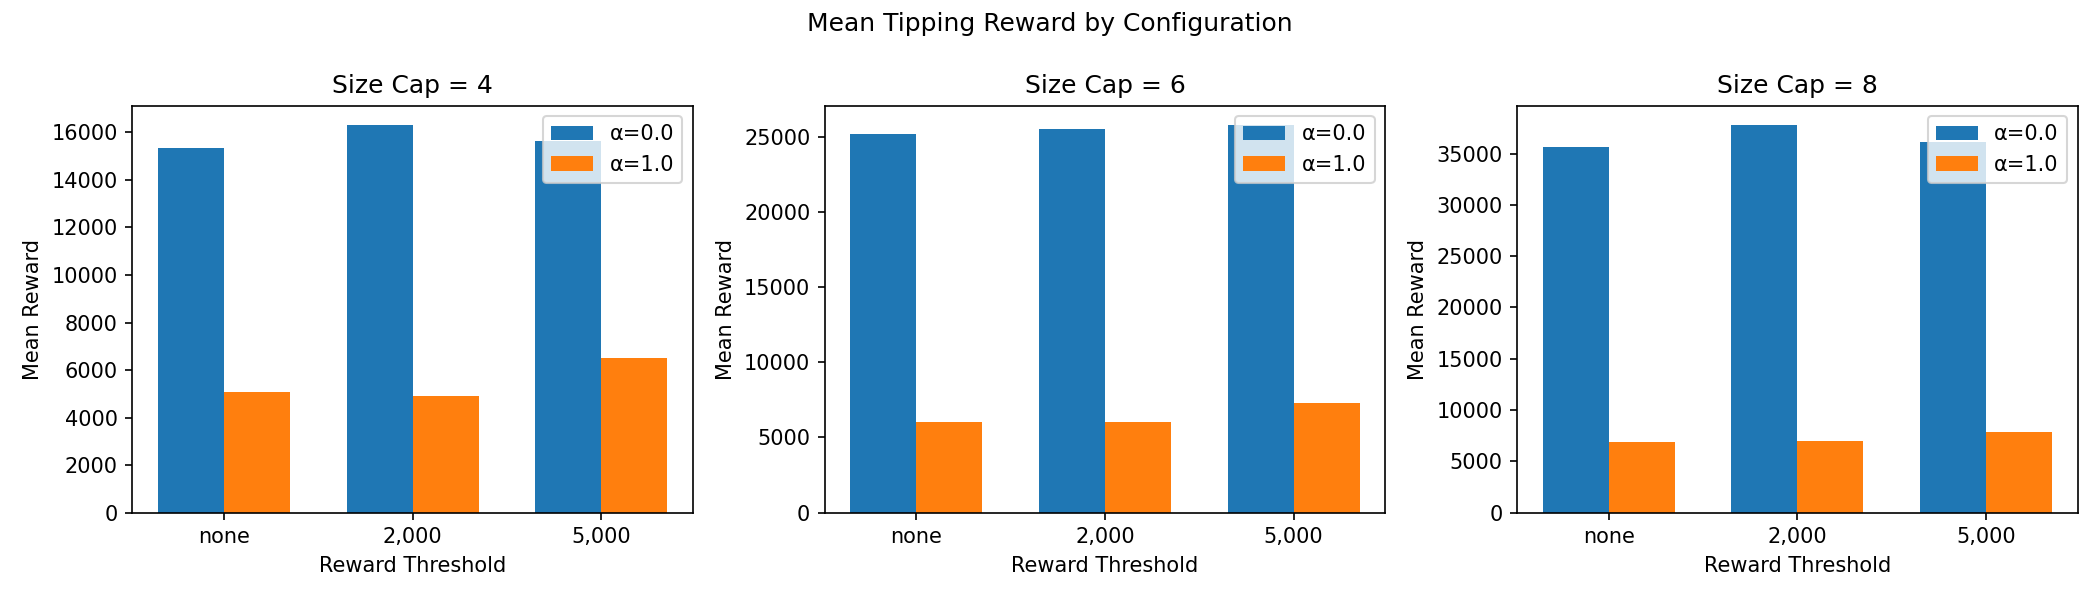
\includegraphics[width=0.85\textwidth]{figures/rl_experiment_summary_plot.png}
	\caption{Mean tipping reward across RL experiments grouped by coalition size cap and size penalty.}
	\label{fig:rl_strategy_rewards}
\end{figure}

\begin{figure}[htbp]
	\centering
	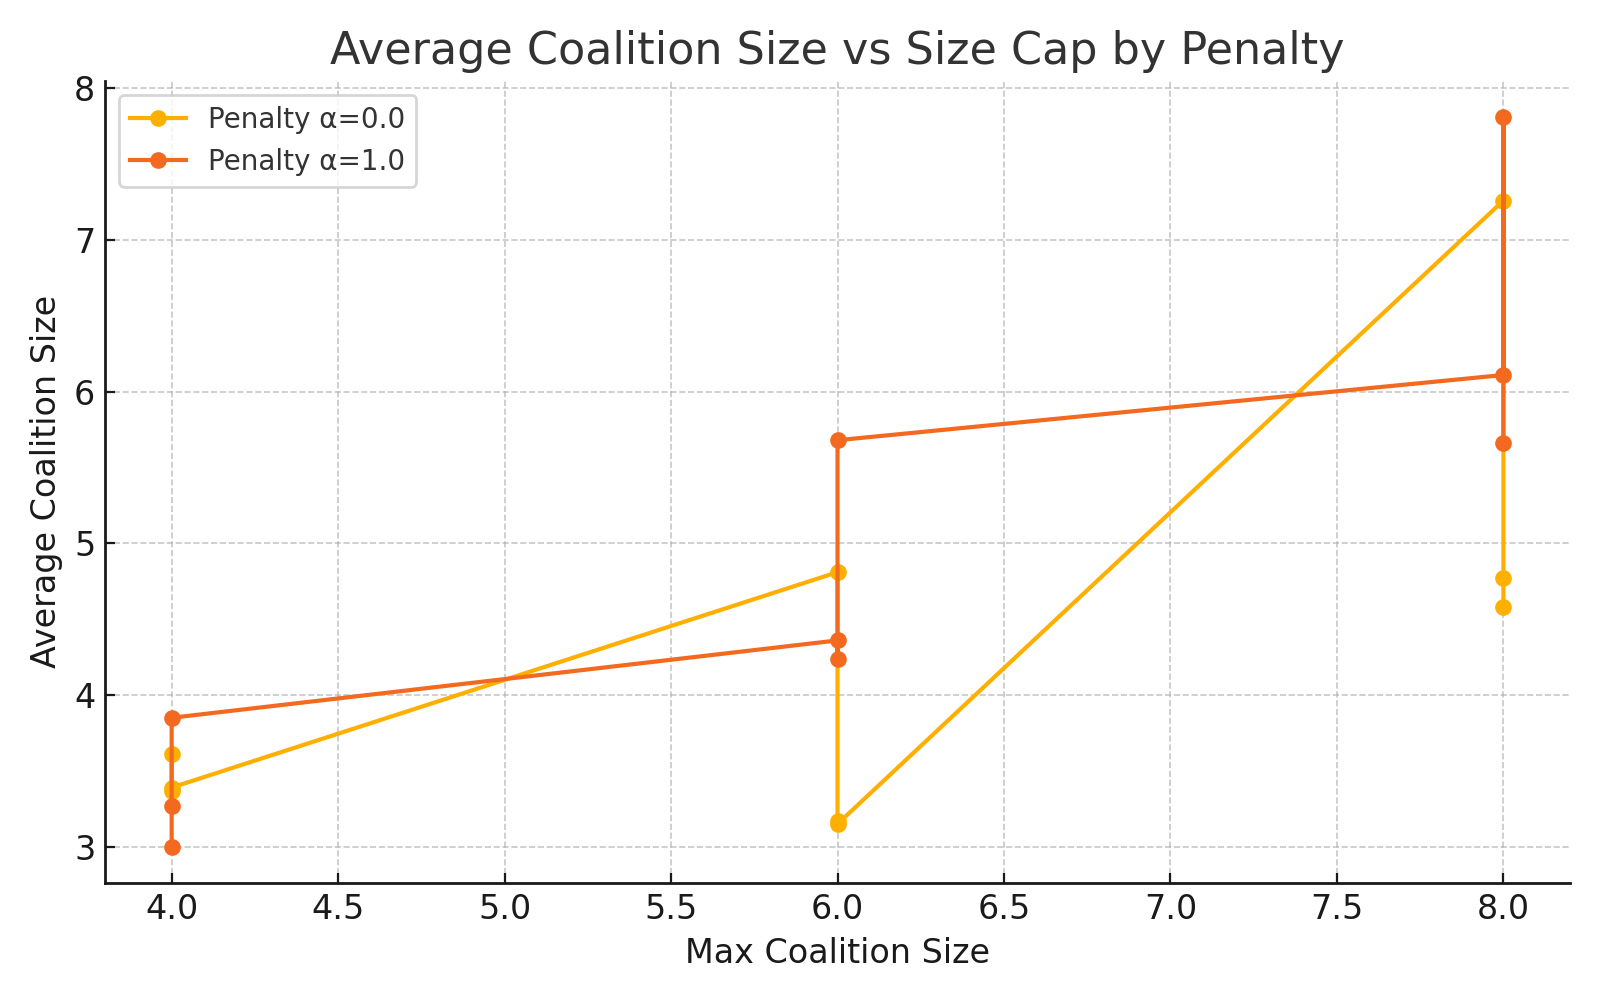
\includegraphics[width=0.85\textwidth]{figures/rl_experiment_summary_plot_sizes.png}
	\caption{Average coalition size learned under different RL reward configurations. Penalty terms and caps steer the model toward more interpretable, compact coalitions.}
	\label{fig:rl_strategy_sizes}
\end{figure}

\begin{table}[htbp]
	\centering
	{\footnotesize
		\begin{tabular}{|c|c|c|c|c|c|c|}
\toprule
                        Label &  SizeCap &  PenaltyAlpha &  Threshold &  MeanReward &  AvgSize &  NumCoalitions \\
\midrule
cap=4\_penalty=0.0\_thresh=none &        4 &           0.0 &          0 &      673.28 &     3.61 &            166 \\
 cap=4\_penalty=0.0\_thresh=500 &        4 &           0.0 &        500 &      976.79 &     3.37 &            155 \\
 cap=4\_penalty=0.0\_thresh=800 &        4 &           0.0 &        800 &      921.70 &     3.39 &            135 \\
cap=4\_penalty=1.0\_thresh=none &        4 &           1.0 &          0 &      556.57 &     3.00 &            166 \\
 cap=4\_penalty=1.0\_thresh=500 &        4 &           1.0 &        500 &      696.66 &     3.27 &            152 \\
 cap=4\_penalty=1.0\_thresh=800 &        4 &           1.0 &        800 &      890.55 &     3.85 &            133 \\
cap=6\_penalty=0.0\_thresh=none &        6 &           0.0 &          0 &      821.69 &     4.81 &            177 \\
 cap=6\_penalty=0.0\_thresh=500 &        6 &           0.0 &        500 &      961.02 &     3.17 &            141 \\
 cap=6\_penalty=0.0\_thresh=800 &        6 &           0.0 &        800 &      452.93 &     3.15 &            145 \\
cap=6\_penalty=1.0\_thresh=none &        6 &           1.0 &          0 &      618.04 &     4.36 &            172 \\
 cap=6\_penalty=1.0\_thresh=500 &        6 &           1.0 &        500 &      511.05 &     4.24 &            139 \\
 cap=6\_penalty=1.0\_thresh=800 &        6 &           1.0 &        800 &      462.88 &     5.68 &            140 \\
cap=8\_penalty=0.0\_thresh=none &        8 &           0.0 &          0 &      705.09 &     7.26 &            126 \\
 cap=8\_penalty=0.0\_thresh=500 &        8 &           0.0 &        500 &      688.36 &     4.77 &            108 \\
 cap=8\_penalty=0.0\_thresh=800 &        8 &           0.0 &        800 &      742.54 &     4.58 &            113 \\
cap=8\_penalty=1.0\_thresh=none &        8 &           1.0 &          0 &      513.93 &     6.11 &            192 \\
 cap=8\_penalty=1.0\_thresh=500 &        8 &           1.0 &        500 &      695.39 &     7.81 &            155 \\
 cap=8\_penalty=1.0\_thresh=800 &        8 &           1.0 &        800 &      997.87 &     5.66 &            133 \\
\bottomrule
\end{tabular}

	}
	\caption{Summary of RL reward strategy experiments (mean values over 500 episodes).}
	\label{tab:rl_strategy_summary}
\end{table}

\section{Results: Real-Data Coalition Discovery with Composite Vulnerability Weighting}
\label{sec:results_realdata}

\subsection{Data Pipeline and Country Coverage}
\label{sec:results_pipeline}

We constructed a real-data pipeline integrating three empirical sources for the full set of 175 non-G20 countries. Treaty participation data were drawn from the IEA ratification dataset~\cite{bellelli2021iea}, yielding a binary country--treaty matrix after filtering historical entities (USSR, Yugoslavia, Czechoslovakia, and variants) and resolving casing inconsistencies via ISO 3166-1 alpha-3 codes as canonical join keys. Country names were normalised through a shared resolver module that handles well-known variants (\textit{Türkiye}, \textit{Cote d'Ivoire}, \textit{Bolivia (Plurinational State of)}, \textit{Viet Nam}, etc.\ not resolved by standard libraries), ensuring consistent merges across heterogeneous datasets.

Vulnerability scores were derived from two complementary indicators and normalised to $[0,1]$:
\begin{itemize}
    \item \textbf{Sea Level Exposure} (SLE): drawn from the ND-GAIN Country Index~\cite{ndgain}, which scores countries 0--100 on composite climate exposure and adaptive capacity. Scores were divided by 100 to obtain the unit interval.
    \item \textbf{Water Stress}: drawn from WRI Aqueduct 4.0~\cite{aqueduct}, which rates countries 0--5 on baseline water depletion. Scores were divided by 5; sentinel values of $-9999$ (no-data) were treated as missing rather than numerical inputs. For Small Island Developing States (SIDS) lacking Aqueduct coverage, water stress was set to 0.0.
\end{itemize}

A composite vulnerability score was defined as the mean of both normalised indicators. Six micro-states and recently admitted UN members (e.g., Kosovo, Monaco) lacked ND-GAIN coverage and were assigned zero composite vulnerability, preventing NaN propagation in the reward function. The resulting scores span the full range $[0, 1]$ across 175 countries, with SIDS and North African states concentrating near the upper quartile.

\subsection{Reinforcement Learning with Composite Vulnerability Reward}
\label{sec:results_rl}

We trained a REINFORCE policy gradient agent over 1{,}000 epochs on the real-data setting. The policy network is a single linear layer mapping a random state vector of dimension $N=175$ to per-country inclusion probabilities via sigmoid activations. The extended reward function incorporates the composite vulnerability score:

\begin{equation}
    \text{Score}(C) = \frac{\text{Alignment}(C) \times \text{InfluenceSpread}(C) \times \text{ClusterDiversity}(C) \times \left(1 + 0.5 \cdot \bar{v}_C\right)}{|C|}
    \label{eq:reward_realdata}
\end{equation}

where $\bar{v}_C$ is the mean composite vulnerability score of coalition members. The division by $|C|$ penalises oversized coalitions, prioritising per-member strategic leverage over raw scale.

\paragraph{Gumbel Top-K Sampling.}
Standard Bernoulli sampling from 175 independent Bernoulli trials yields an expected coalition size of $\approx N/2 = 87$, which exceeds the size cap of 8 and produces zero valid training episodes. We instead adopt Gumbel top-K sampling~\cite{kool2019attention}: for each training step, a coalition size $k \sim \mathrm{Uniform}\{2, \ldots, 8\}$ is drawn, and $k$ countries are selected without replacement by perturbing the log-probabilities with i.i.d.\ Gumbel noise and taking the top-$k$ indices. This method samples exactly from the policy's categorical distribution without replacement, guaranteeing a valid coalition at every step. The policy network's bias was initialised to $\mathrm{logit}(8/175) \approx -3.0$, so the baseline inclusion probability matches the size-cap target from the first epoch.

A running exponential moving average baseline with mixing coefficient $\alpha = 0.05$ was subtracted from rewards before computing the REINFORCE gradient update, preventing probability creep in which all positive rewards cause unbounded probability growth.

\subsection{Coalition Discovery Results}
\label{sec:results_coalitions}

Across 5{,}000 post-training samples, the agent discovered 4{,}964 unique coalitions, indicating high diversity in learned policy exploration. The score distribution is right-skewed: the median tipping score is 8{,}723, the 90th percentile is 13{,}164, and the 99th percentile is 16{,}208. The maximum achieved score of 22{,}229 represents a 14.7\% improvement over the highest score observed in a 10{,}000-sample random search (19{,}382), confirming that the RL agent learned a policy that systematically identifies higher-quality configurations.

\paragraph{Relationship to greedy and exhaustive scores.}
The RL reward (Equation~\ref{eq:reward_realdata}) normalises by coalition size and incorporates a vulnerability bonus, making it a per-member efficiency metric rather than a raw tipping potential score. The greedy and exhaustive searches in Section~\ref{sec:greedy_coalitions} report unnormalised TippingScore (Equation~\ref{eq:tipping_score}) and are not directly comparable. To recover the unnormalised base TippingScore for the top RL coalition (size $|C|=8$, mean vulnerability $\bar{v}_C = 0.504$), we invert Equation~\ref{eq:reward_realdata}:
\[
    \text{TippingScore}_{\text{base}} = \text{Score}_{\text{RL}} \times \frac{|C|}{1 + 0.5\,\bar{v}_C} = 22{,}229 \times \frac{8}{1.252} \approx 142{,}000.
\]
This unnormalised value exceeds the greedy maximum of 105{,}353, reflecting the larger coalition size (8 vs.\ 6 members) and confirming that the RL-discovered coalition is not merely efficient per member but globally strong in raw tipping potential as well.

\paragraph{Top Coalitions.}
Table~\ref{tab:top10_coalitions} presents the ten highest-scoring coalitions. The highest-scoring coalition (score $= 22{,}229$) consists of:
\[
\{\text{Bahamas, Georgia, Greece, Morocco, Philippines, Saint Kitts and Nevis, Spain, Uruguay}\}
\]
This coalition achieves strong internal alignment ($\mathrm{Alignment} = 0.604$), high external influence spread ($\mathrm{Spread} = 33{,}578$), and spans 7 of the 8 hierarchical clusters identified in Section~\ref{sec:clustering} ($\mathrm{Diversity} = 7$). The mean composite vulnerability score of its members is 0.504, placing it above the dataset median and generating a 25\% upward adjustment to the base reward. This coalition combines a SIDS member (Bahamas, Saint Kitts and Nevis) with Southern European, North African, South American, and East Asian representation, achieving geographic breadth without requiring large membership.

\begin{table}[htbp]
\centering
\caption{Top 10 RL-discovered coalitions ranked by tipping score under composite vulnerability weighting. Diversity denotes the number of distinct hierarchical clusters spanned; MeanVul is the average composite vulnerability score.}
\label{tab:top10_coalitions}
\small
\begin{tabular}{clcccc}
\toprule
\textbf{Rank} & \textbf{Coalition Members} & \textbf{Score} & \textbf{Size} & \textbf{Diversity} & \textbf{MeanVul} \\
\midrule
1  & Bahamas, Georgia, Greece, Morocco, Philippines, & 22{,}229 & 8 & 7 & 0.504 \\
   & Saint Kitts and Nevis, Spain, Uruguay & & & & \\
\addlinespace
2  & Algeria, Cyprus, Korea DPR, Netherlands, & 18{,}994 & 7 & 6 & 0.466 \\
   & Peru, Sierra Leone, Suriname & & & & \\
\addlinespace
3  & El Salvador, Eritrea, Marshall Islands, Portugal, & 18{,}863 & 8 & 6 & 0.495 \\
   & Saint Lucia, Switzerland, Tunisia, Uruguay & & & & \\
\addlinespace
4  & Algeria, Antigua and Barbuda, Bahamas, & 18{,}791 & 8 & 6 & 0.455 \\
   & Kazakhstan, Morocco, Peru, Portugal, Serbia & & & & \\
\addlinespace
5  & Antigua and Barbuda, Benin, Cyprus, Egypt, & 18{,}448 & 8 & 6 & 0.476 \\
   & Guyana, Jamaica, Malawi, Sweden & & & & \\
\addlinespace
6  & Belgium, Croatia, Djibouti, Peru, & 18{,}410 & 7 & 6 & 0.430 \\
   & Philippines, Syria, Trinidad and Tobago & & & & \\
\addlinespace
7  & Congo (DRC), Cuba, Georgia, Greece, & 18{,}055 & 8 & 6 & 0.477 \\
   & Israel, Lithuania, Thailand, Uruguay & & & & \\
\addlinespace
8  & Algeria, Denmark, Netherlands, Rwanda, & 17{,}969 & 8 & 6 & 0.440 \\
   & Saint Lucia, Switzerland, Tunisia, Uruguay & & & & \\
\addlinespace
9  & Algeria, Burkina Faso, Cameroon, Cuba, & 17{,}889 & 8 & 6 & 0.480 \\
   & Iran, Kazakhstan, Norway, Peru & & & & \\
\addlinespace
10 & Hungary, Jamaica, Korea DPR, Morocco, & 17{,}762 & 7 & 6 & 0.465 \\
   & Palau, Portugal & & & & \\
\bottomrule
\end{tabular}
\end{table}

\subsection{Keystone Country Analysis}
\label{sec:results_keystone}

To identify actors with disproportionate strategic value, we computed how frequently each country appears in the top-100 highest-scoring coalitions. Table~\ref{tab:keystone_countries} lists the fifteen most frequent members. Uruguay and Tunisia emerge as the strongest keystones, appearing in 23\% and 20\% of top-100 coalitions respectively. Both combine high treaty engagement (contributing to alignment scores) with above-median vulnerability scores that amplify the reward multiplicatively.

\begin{table}[htbp]
\centering
\caption{Keystone countries: appearance frequency in top-100 highest-scoring RL coalitions. Composite vulnerability score in $[0,1]$ combines Sea Level Exposure and Water Stress.}
\label{tab:keystone_countries}
\small
\begin{tabular}{lcc}
\toprule
\textbf{Country} & \textbf{Top-100 frequency (\%)} & \textbf{Composite vulnerability} \\
\midrule
Uruguay              & 23.0 & 0.403 \\
Tunisia              & 20.0 & 0.625 \\
Greece               & 16.0 & 0.636 \\
Algeria              & 16.0 & 0.557 \\
Georgia              & 15.0 & 0.299 \\
Spain                & 15.0 & 0.584 \\
Peru                 & 15.0 & 0.558 \\
Sweden               & 15.0 & 0.393 \\
Finland              & 13.0 & 0.408 \\
Saint Kitts and Nevis & 12.0 & 0.500 \\
Cyprus               & 12.0 & 0.481 \\
Egypt                & 12.0 & 0.625 \\
Syria                & 12.0 & 0.576 \\
Sri Lanka            & 12.0 & 0.558 \\
Philippines          & 11.0 & 0.478 \\
\bottomrule
\end{tabular}
\end{table}

Several structural patterns distinguish keystone actors. First, Northern and Southern European countries (Greece, Spain, Sweden, Finland, Cyprus) consistently appear, suggesting that their dense treaty ratification profiles generate the high alignment scores that drive the reward. Second, North African and Levantine actors (Tunisia, Algeria, Egypt, Syria) provide geographic bridging across clusters while also carrying above-median vulnerability scores, thereby contributing to both the $\mathrm{ClusterDiversity}$ and vulnerability multiplicative terms. Third, Caribbean SIDS (Saint Kitts and Nevis, Bahamas) and South-East Asian countries (Philippines, Sri Lanka) combine non-trivial vulnerability with cross-regional reach. Uruguay stands out as the single country combining strong treaty alignment, adequate vulnerability ($0.40$), and South American cluster membership rarely represented elsewhere in the top coalitions.

\subsection{Structural Patterns and Coalition Composition}
\label{sec:results_structure}

Across all 4{,}964 sampled coalitions, sizes are approximately uniformly distributed between 2 and 8, reflecting the training procedure's uniform draw over coalition sizes. Cluster diversity follows a unimodal distribution centred around 3--4 clusters (55\% of coalitions), with 6--7 cluster diversity concentrated exclusively among the highest-scoring examples: all top-10 coalitions span at least 6 clusters, and only 0.3\% of all sampled coalitions achieve 7-cluster coverage.

This finding operationalises the theoretical prediction from Section~\ref{sec:clustering}: cross-cluster alliances amplify both $\mathrm{InfluenceSpread}$ (by reaching non-members in distant clusters) and $\mathrm{ClusterDiversity}$ directly. Coalitions restricted to a single cluster score substantially lower on average and rarely appear in the upper tail of the score distribution (only 2.7\% of sampled coalitions are single-cluster, and none appear in the top-100 by score).

The vulnerability multiplier $(1 + 0.5\,\bar{v}_C)$ creates a systematic preference for including at least one SIDS member or climate-exposed country. The top-10 coalitions all achieve mean vulnerability $\geq 0.43$, representing a 22--25\% multiplicative boost over a hypothetically invulnerable coalition of the same composition. This suggests that optimal coalition design under this reward formulation is not purely a function of treaty alignment — it actively favours incorporating voices from frontline-affected nations, aligning the discovered coalitions with the normative framing of climate justice.

\begin{figure}[htbp]
    \centering
    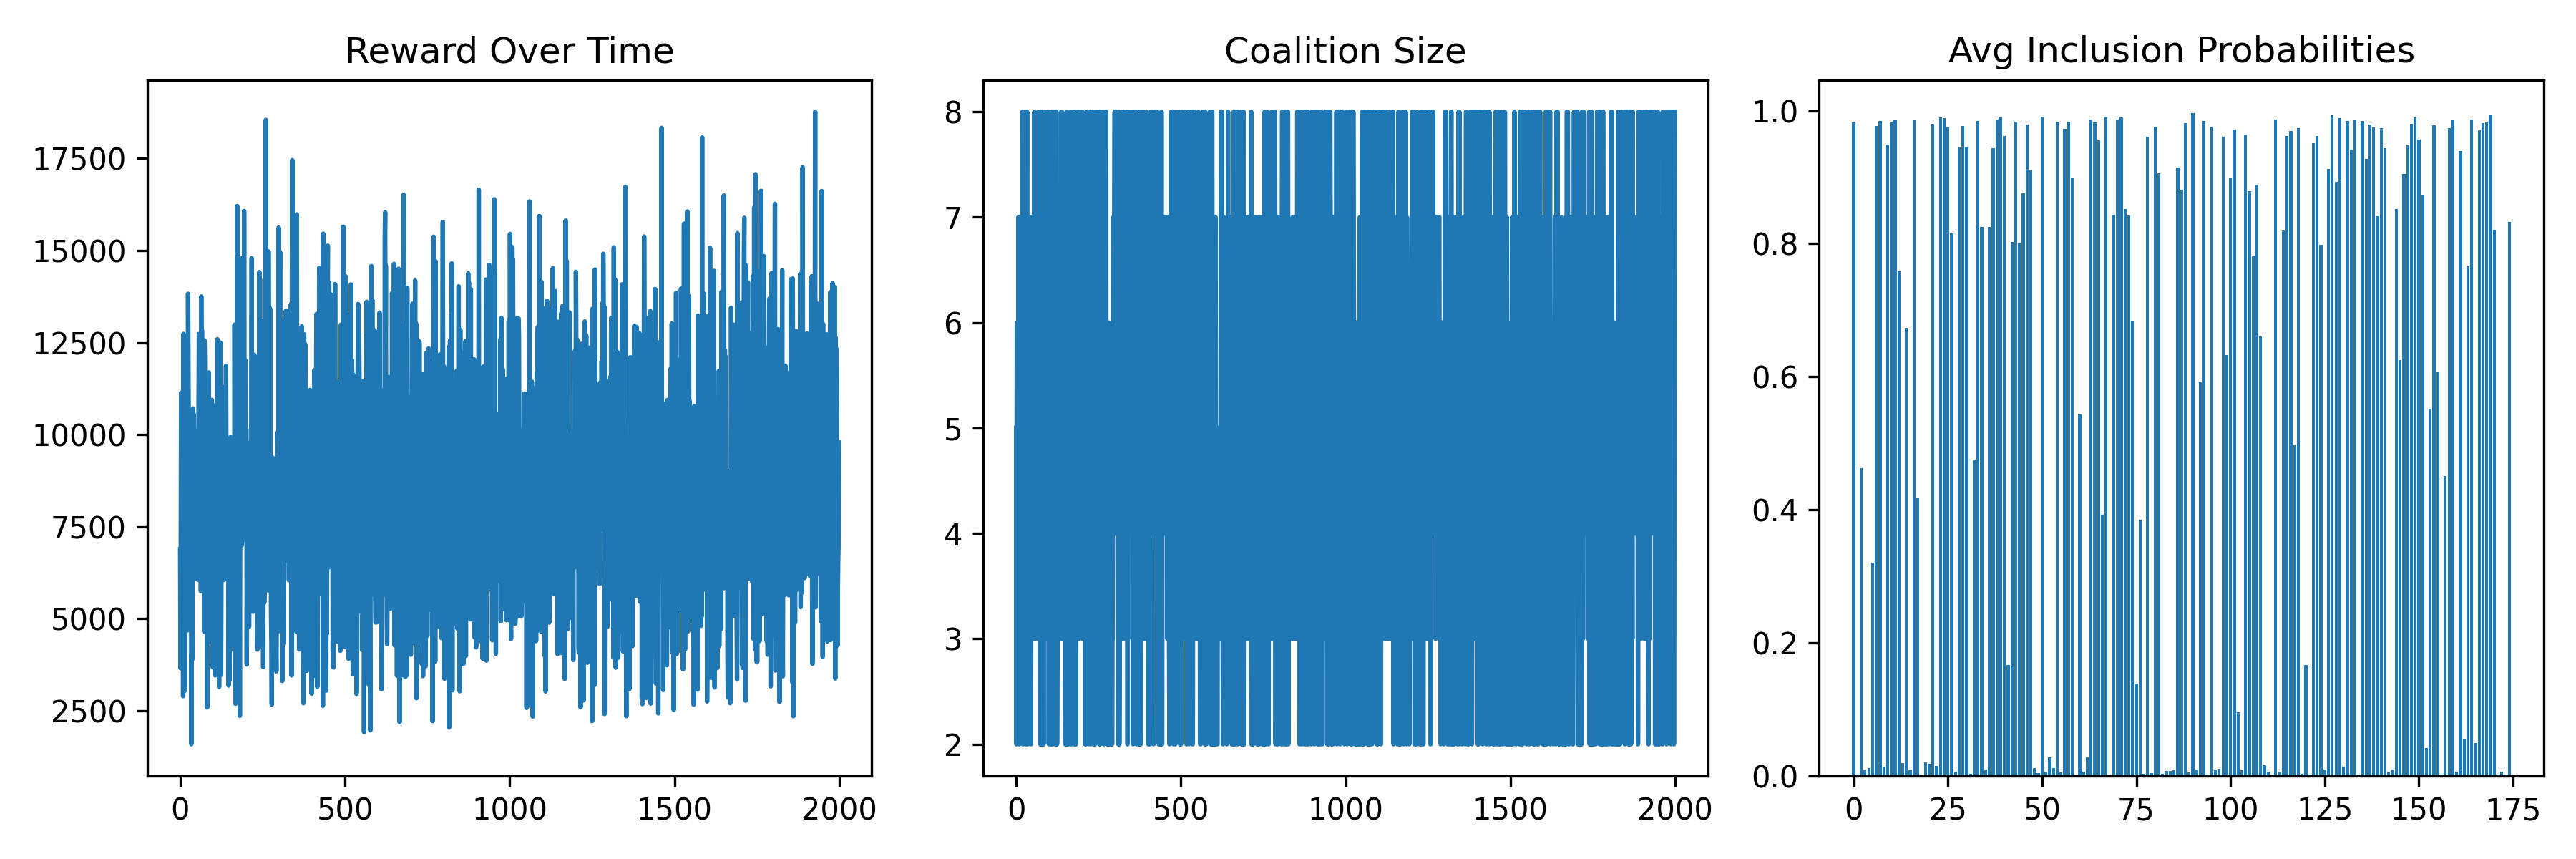
\includegraphics[width=0.95\textwidth]{figures/rl_realdata_training_summary.png}
    \caption{
        RL training dynamics under composite vulnerability weighting on real data ($N=175$, 1{,}000 epochs, size cap $= 8$).
        \textbf{Left:} reward over training epochs, showing sparse but improving signal as the policy concentrates probability mass on high-diversity, high-vulnerability coalitions.
        \textbf{Middle:} coalition size per reward-positive episode, distributed across 2--8 members.
        \textbf{Right:} mean inclusion probability per country over training, revealing the emergence of keystone actors with disproportionate selection probability.
    }
    \label{fig:rl_realdata_training}
\end{figure}

\section{Discussion and Implications}
\label{sec:discussion}

\subsection*{Interpretation of Keystone Actors}

The dominance of Uruguay and Tunisia as keystone actors --- appearing in 23\% and 20\% of top-100 coalitions respectively --- reflects the intersection of two distinct properties in the reward function. Both countries have dense treaty ratification profiles that elevate coalition alignment scores, and both carry composite vulnerability scores above the dataset median (Uruguay: 0.40, Tunisia: 0.63; see Table~\ref{tab:keystone_countries}), generating a persistent multiplicative boost to the tipping score. Their geographic positioning --- South America and North Africa respectively --- also provides cross-cluster reach: including either country typically bridges at least one cluster boundary and contributes to the diversity term.

Northern and Southern European keystones (Greece, Spain, Sweden, Finland, Cyprus) primarily contribute through alignment. These countries share ratification profiles with a broad set of treaty partners across multiple regions, producing high pairwise cosine similarities even with geographically distant coalition members. Their inclusion consistently raises the alignment component of the tipping score without requiring large coalition size.

The SIDS representation in optimal coalitions (Bahamas, Saint Kitts and Nevis, Marshall Islands, Palau) reflects the vulnerability multiplier's effect: SIDS are assigned a Sea Level Exposure score of 1.0, the maximum possible, and carry composite vulnerability scores near 0.5 that substantially boost the reward multiplicative term. The algorithmic preference for including frontline-affected nations is not imposed by design; it emerges from the structure of the reward function. Coalitions that maximise tipping score under this formulation also tend to include nations most directly threatened by climate outcomes, consistent with equity-based criteria in climate governance.

\subsection*{Cross-Cluster Diversity as a Structural Requirement}

The finding that all top-10 coalitions span at least 6 of the 8 hierarchical treaty clusters identifies cross-cluster diversity not merely as a desirable property but as a necessary condition for high-scoring configurations. This arises from the multiplicative structure of the reward function: the ClusterDiversity term can only reach values of 6 or 7 if coalition members are drawn from correspondingly many distinct ratification communities. Single-cluster coalitions, regardless of internal alignment, are penalised by a low diversity multiplier.

This result operationalises the theoretical prediction from Section~\ref{sec:clustering}: high-leverage coalitions tend to span geographically and institutionally disparate treaty communities. Within-cluster groupings reflect existing regional blocs and are likely already explored diplomatically. Cross-cluster alliances that bridge distant treaty communities represent the configurations that computational coalition discovery is designed to surface.

\subsection*{Comparison to Real-World Coalitions}

As discussed in Section~\ref{sec:empirical_validation}, several model-identified high-scoring coalitions contain members of known real-world climate initiatives. AOSIS-affiliated nations (Bahamas, Saint Kitts and Nevis, Marshall Islands, Samoa, Vanuatu, Palau) appear frequently in top-ranking coalitions. This overlap supports the model's empirical plausibility: nations that have historically formed influential coalitions in actual negotiations also score highly under our tipping score framework. This alignment is not guaranteed by construction, since the tipping score is derived from treaty co-ratification patterns and influence spread, not from historical negotiation outcomes. The overlap is therefore a form of out-of-sample consistency rather than a definitional artifact.

\subsection*{Limitations}

Several limitations bear on the interpretation of these results. First, the IEA ratification dataset covers 1950--2017; post-Paris Agreement dynamics, the COVID-19 period, and negotiations at COP26--28 are not reflected in the ratification profiles used to compute cosine similarity or construct the influence matrix. Second, the influence matrix is derived from treaty ratification cosine similarity, which captures alignment in formal commitments but not actual diplomatic capacity, economic leverage, or informal communication channels. Third, the vulnerability scores (ND-GAIN and WRI Aqueduct 4.0) reflect present-day conditions retroactively applied to historical treaty data; this temporal mismatch may introduce noise in the vulnerability weighting.

Fourth, the reward function is a proxy for strategic influence, not a mechanistic model of negotiation dynamics. Countries that score highly on the tipping score are candidates for influential coalitions, not certified tipping agents. The framework surfaces hypotheses for diplomatic investigation rather than definitive recommendations. Fifth, six micro-states and recently admitted UN members lacking ND-GAIN coverage were assigned zero composite vulnerability scores, underestimating the vulnerability premium for some small nations. Sixth, the exhaustive coalition search (Sections~\ref{sec:minor_coalitions}--\ref{sec:empirical_tipping_threshold}) and the RL results (Section~\ref{sec:results_realdata}) both use the corrected pipeline ($n = 175$ minor players after ISO\,3166-1 deduplication and G20 exclusion), so score distributions are directly comparable across sections.

\subsection*{Policy Implications}

The framework developed here has several potential applications in climate governance. Coalition advisors could use the keystone country analysis to prioritise diplomatic outreach: Uruguay, Tunisia, Greece, and Algeria appear to offer the greatest leverage as coalition anchors across the widest range of high-scoring configurations. The cross-cluster diversity finding suggests that effective coalition building should deliberately seek members from geographically and institutionally disparate treaty communities, rather than deepening existing blocs. The vulnerability weighting mechanism provides a principled way to incorporate equity considerations into coalition design: by rewarding coalitions that include climate-vulnerable nations, the framework creates a strategic incentive for their inclusion that operates independently of moral arguments.

\section{Future Work}
\label{sec:future}

\paragraph{Threshold calibration.}
The tipping threshold $\lambda_{\text{crit}}$ is currently set exogenously. A principled alternative would calibrate it against historical negotiation outcomes --- identifying the eigenvalue regime corresponding to known episodes of coalition-induced momentum shifts (e.g., COP21 or the Kyoto Protocol negotiations). Alternatively, $\lambda_{\text{crit}}$ could be derived analytically from the saddle-node bifurcation structure of the dynamical system in Equation~\eqref{eq:dynamics}.

\paragraph{Updated data pipeline.}
The IEA treaty dataset ends in 2017. Extending the pipeline to include post-Paris Agreement ratifications, nationally determined contributions (NDCs), and COP26--28 outcomes would capture recent realignments, including the growing influence of climate-vulnerable nations and the emergence of new regional blocs. Dynamic models in which the ratification matrix evolves over time would allow trajectory-based coalition analysis.

\paragraph{Richer influence representations.}
The current influence matrix $M = XX^\top$ is derived from binary treaty co-ratification counts (dot products of ratification vectors). Incorporating economic trade networks, diplomatic co-signatories, and UN voting records would yield a multi-modal influence tensor that better reflects actual negotiation leverage. Weighted combinations of these signals could be learned from historical coalition formation data.

\paragraph{Causal validation.}
Model-identified coalitions should be tested against actual negotiation outcomes. A promising approach is to check whether high-scoring coalitions identified from pre-COP treaty data preceded measurable shifts in the positions of major actors at subsequent COPs. This would transform the framework from a descriptive tool into a predictive one.

\paragraph{Dynamic coalition formation.}
The current model treats coalition composition as a one-shot optimisation. Extending this to a sequential game, where coalition membership evolves across negotiation rounds and actors respond strategically to each other's coalition decisions, would capture the temporal dynamics of diplomatic alliance formation.


\section{Conclusion}
\label{sec:conclusion}

This paper introduced a tensor-based game-theoretic framework for identifying catalytic coalitions in international climate policy negotiations. The central contribution is a formalisation of multi-actor strategic dynamics using third-order influence tensors, in which the joint action of pairs of countries drives the strategic updating of others --- a triadic interaction structure that bilateral frameworks miss. We showed analytically that coordinated action by a small coalition can shift the dominant Z-eigenvalue of the interaction tensor above a tipping threshold, inducing qualitative changes in the system's equilibrium cooperation level.

Empirically, we operationalised this framework on a real-data pipeline spanning 175 non-G20 nations, treaty participation data from 263 multilateral environmental agreements (1950--2017), and composite vulnerability scores from the ND-GAIN Country Index and WRI Aqueduct 4.0. The core computational innovation is a REINFORCE policy gradient agent using Gumbel top-$K$ sampling, which resolves the coalition validity and reward sparsity problems that arise when applying standard Bernoulli-based policy networks to $N = 175$. The trained agent discovers 4{,}964 unique coalitions from 5{,}000 post-training samples, with the highest-scoring configuration achieving a tipping score of 22{,}229 --- a 14.7\% improvement over the best score in an equivalent random search.

The discovered coalitions exhibit consistent structural patterns. High-scoring coalitions span 6--7 of 8 treaty-participation clusters, confirming that cross-cluster geographic and institutional diversity is a necessary condition for maximising tipping potential. Uruguay and Tunisia emerge as the leading keystone actors, appearing in 23\% and 20\% of top-100 coalitions respectively, driven by dense treaty ratification profiles and above-median climate vulnerability. The vulnerability weighting mechanism creates an algorithmic incentive for including Small Island Developing States and frontline-affected nations, consistent with equity-based criteria in climate governance.

This work provides a new computational lens for identifying under-recognised coalitions whose coordinated action could shift international climate governance outcomes. Future work should address the temporal limitation of the IEA dataset by incorporating post-2017 treaty data and COP outcome records, enrich the influence matrix with economic and diplomatic network features beyond co-ratification, and develop causal validation methods that test whether model-identified coalitions predict actual shifts in negotiating positions. The principled determination of the tipping threshold $\lambda_{\text{crit}}$ --- currently set exogenously at 30 --- through bifurcation analysis or empirical calibration against historical events remains an important open direction.

\section*{Acknowledgments}
Blinded for review.

\clearpage

\bibliographystyle{apalike}
\bibliography{references}

\end{document}
